%% LyX 2.4.3 created this file.  For more info, see https://www.lyx.org/.
%% Do not edit unless you really know what you are doing.
\documentclass[journal,article,submit,pdftex,moreauthors]{Definitions/mdpi}
\usepackage{textcomp}
\usepackage[utf8]{inputenc}
\usepackage{array}
\usepackage{float}
\usepackage{url}
\usepackage{multirow}
\usepackage{varwidth}
\usepackage{amsmath}
\usepackage{graphicx}
\usepackage{rotfloat}

\makeatletter

%%%%%%%%%%%%%%%%%%%%%%%%%%%%%% LyX specific LaTeX commands.

\Title{The Echo Optimizer: A Novel Metaheuristic Inspired by Acoustic Reflection
Principles}

\TitleCitation{The Echo Optimizer: A Novel Metaheuristic Inspired by Acoustic Reflection
Principles}

\Author{Vasileios Charilogis$^{1}$, Ioannis G. Tsoulos$^{2,*}$ }

\AuthorNames{Vasileios Charilogis, Ioannis G. Tsoulos }

\AuthorNames{Charilogis, V.; Tsoulos, I.G. }


\address{$^{1}$\quad{}Department of Informatics and Telecommunications,
University of Ioannina, 47150 Kostaki Artas, Greece; v.charilog@uoi.gr\\
$^{2}$\quad{}Department of Informatics and Telecommunications, University
of Ioannina, 47150 Kostaki Artas, Greece; itsoulos@uoi.gr}


\corres{Correspondence: itsoulos@uoi.gr}


\abstract{The Echo Optimizer Method is an innovative optimization technique
inspired by the natural behavior of sound echoes. It is based on generating
modified solutions (echoes) that combine directed reflection toward
the best-known solution and random noise that attenuates over time.
The method introduces two groundbreaking mechanisms to enhance performance:
an approximate evaluation system that avoids costly computations for
unpromising solutions, and an echo memory that stores and reuses past
evaluations. These mechanisms enable a significant reduction in computational
resources (up to 40--60\% fewer evaluations) while maintaining the
method's effectiveness. The Echo Optimizer excels in balancing exploration
of the solution space with exploitation of the best-known solutions,
demonstrating impressive performance in problems with numerous local
minima and high dimensionality. Experimental tests on standard optimization
problems have shown faster convergence and reduced result variability
compared to classical methods, making it a highly attractive choice
for various optimization challenges, particularly in cases where evaluating
the objective function is computationally expensive.}


\keyword{Optimization; Echo Optimizer; Evolutionary Algorithms; Global Optimization;
Adaptive Termination; Mutation Strategies; Metaheuristics;}

\newcommand*\LyXZeroWidthSpace{\hspace{0pt}}
\DeclareTextSymbolDefault{\textquotedbl}{T1}
%% Because html converters don't know tabularnewline
\providecommand{\tabularnewline}{\\}
%% Variable width box for table cells
\newenvironment{cellvarwidth}[1][t]
    {\begin{varwidth}[#1]{\linewidth}}
    {\@finalstrut\@arstrutbox\end{varwidth}}
\floatstyle{ruled}
\newfloat{algorithm}{tbp}{loa}
\providecommand{\algorithmname}{Algorithm}
\floatname{algorithm}{\protect\algorithmname}

%%%%%%%%%%%%%%%%%%%%%%%%%%%%%% User specified LaTeX commands.
%  LaTeX support: latex@mdpi.com 
%  For support, please attach all files needed for compiling as well as the log file, and specify your operating system, LaTeX version, and LaTeX editor.

%=================================================================
%\documentclass[preprints,article,submit,pdftex,moreauthors]{Definitions/mdpi} 
% For posting an early version of this manuscript as a preprint, you may use "preprints" as the journal. Changing "submit" to "accept" before posting will remove line numbers.

% Below journals will use APA reference format:
% admsci, aichem, behavsci, businesses, econometrics, economies, education, ejihpe, famsci, games, humans, ijcs, ijfs, journalmedia, jrfm, languages, psycholint, publications, tourismhosp, youth

% Below journals will use Chicago reference format:
% arts, genealogy, histories, humanities, jintelligence, laws, literature, religions, risks, socsci

%--------------------
% Class Options:
%--------------------
%----------
% journal
%----------
% Choose between the following MDPI journals:
% accountaudit, acoustics, actuators, addictions, adhesives, admsci, adolescents, aerobiology, aerospace, agriculture, agriengineering, agrochemicals, agronomy, ai, air, algorithms, allergies, alloys, amh, analytica, analytics, anatomia, anesthres, animals, antibiotics, antibodies, antioxidants, applbiosci, appliedchem, appliedmath, appliedphys, applmech, applmicrobiol, applnano, applsci, aquacj, architecture, arm, arthropoda, arts, asc, asi, astronomy, atmosphere, atoms, audiolres, automation, axioms, bacteria, batteries, bdcc, behavsci, beverages, biochem, bioengineering, biologics, biology, biomass, biomechanics, biomed, biomedicines, biomedinformatics, biomimetics, biomolecules, biophysica, biosensors, biosphere, biotech, birds, blockchains, bloods, blsf, brainsci, breath, buildings, businesses, cancers, carbon, cardiogenetics, catalysts, cells, ceramics, challenges, chemengineering, chemistry, chemosensors, chemproc, children, chips, cimb, civileng, cleantechnol, climate, clinbioenerg, clinpract, clockssleep, cmd, cmtr, coasts, coatings, colloids, colorants, commodities, complications, compounds, computation, computers, condensedmatter, conservation, constrmater, cosmetics, covid, crops, cryo, cryptography, crystals, csmf, ctn, curroncol, cyber, dairy, data, ddc, dentistry, dermato, dermatopathology, designs, devices, diabetology, diagnostics, dietetics, digital, disabilities, diseases, diversity, dna, drones, dynamics, earth, ebj, ecm, ecologies, econometrics, economies, education, eesp, ejihpe, electricity, electrochem, electronicmat, electronics, encyclopedia, endocrines, energies, eng, engproc, ent, entomology, entropy, environments, epidemiologia, epigenomes, esa, est, famsci, fermentation, fibers, fintech, fire, fishes, fluids, foods, forecasting, forensicsci, forests, fossstud, foundations, fractalfract, fuels, future, futureinternet, futureparasites, futurepharmacol, futurephys, futuretransp, galaxies, games, gases, gastroent, gastrointestdisord, gastronomy, gels, genealogy, genes, geographies, geohazards, geomatics, geometry, geosciences, geotechnics, geriatrics, glacies, grasses, greenhealth, gucdd, hardware, hazardousmatters, healthcare, hearts, hemato, hematolrep, heritage, higheredu, highthroughput, histories, horticulturae, hospitals, humanities, humans, hydrobiology, hydrogen, hydrology, hygiene, idr, iic, ijerph, ijfs, ijgi, ijmd, ijms, ijns, ijpb, ijt, ijtm, ijtpp, ime, immuno, informatics, information, infrastructures, inorganics, insects, instruments, inventions, iot, j, jal, jcdd, jcm, jcp, jcs, jcto, jdad, jdb, jeta, jfb, jfmk, jimaging, jintelligence, jlpea, jmahp, jmmp, jmms, jmp, jmse, jne, jnt, jof, joitmc, joma, jop, jor, journalmedia, jox, jpbi, jpm, jrfm, jsan, jtaer, jvd, jzbg, kidney, kidneydial, kinasesphosphatases, knowledge, labmed, laboratories, land, languages, laws, life, lights, limnolrev, lipidology, liquids, literature, livers, logics, logistics, lubricants, lymphatics, machines, macromol, magnetism, magnetochemistry, make, marinedrugs, materials, materproc, mathematics, mca, measurements, medicina, medicines, medsci, membranes, merits, metabolites, metals, meteorology, methane, metrics, metrology, micro, microarrays, microbiolres, microelectronics, micromachines, microorganisms, microplastics, microwave, minerals, mining, mmphys, modelling, molbank, molecules, mps, msf, mti, multimedia, muscles, nanoenergyadv, nanomanufacturing, nanomaterials, ncrna, ndt, network, neuroglia, neurolint, neurosci, nitrogen, notspecified, nursrep, nutraceuticals, nutrients, obesities, oceans, ohbm, onco, oncopathology, optics, oral, organics, organoids, osteology, oxygen, parasites, parasitologia, particles, pathogens, pathophysiology, pediatrrep, pets, pharmaceuticals, pharmaceutics, pharmacoepidemiology, pharmacy, philosophies, photochem, photonics, phycology, physchem, physics, physiologia, plants, plasma, platforms, pollutants, polymers, polysaccharides, populations, poultry, powders, preprints, proceedings, processes, prosthesis, proteomes, psf, psych, psychiatryint, psychoactives, psycholint, publications, purification, quantumrep, quaternary, qubs, radiation, reactions, realestate, receptors, recycling, regeneration, religions, remotesensing, reports, reprodmed, resources, rheumato, risks, robotics, rsee, ruminants, safety, sci, scipharm, sclerosis, seeds, sensors, separations, sexes, signals, sinusitis, siuj, skins, smartcities, sna, societies, socsci, software, soilsystems, solar, solids, spectroscj, sports, standards, stats, std, stresses, surfaces, surgeries, suschem, sustainability, symmetry, synbio, systems, tae, targets, taxonomy, technologies, telecom, test, textiles, thalassrep, therapeutics, thermo, timespace, tomography, tourismhosp, toxics, toxins, transplantology, transportation, traumacare, traumas, tropicalmed, universe, urbansci, uro, vaccines, vehicles, venereology, vetsci, vibration, virtualworlds, viruses, vision, waste, water, wem, wevj, wild, wind, women, world, youth, zoonoticdis

%---------
% article
%---------
% The default type of manuscript is "article", but can be replaced by: 
% abstract, addendum, article, book, bookreview, briefreport, casereport, comment, commentary, communication, conferenceproceedings, correction, conferencereport, entry, expressionofconcern, extendedabstract, datadescriptor, editorial, essay, erratum, hypothesis, interestingimage, obituary, opinion, projectreport, reply, retraction, review, perspective, protocol, shortnote, studyprotocol, systematicreview, supfile, technicalnote, viewpoint, guidelines, registeredreport, tutorial
% supfile = supplementary materials

%----------
% submit
%----------
% The class option "submit" will be changed to "accept" by the Editorial Office when the paper is accepted. This will only make changes to the frontpage (e.g., the logo of the journal will get visible), the headings, and the copyright information. Also, line numbering will be removed. Journal info and pagination for accepted papers will also be assigned by the Editorial Office.

%------------------
% moreauthors
%------------------
% If there is only one author the class option oneauthor should be used. Otherwise use the class option moreauthors.

%---------
% pdftex
%---------
% The option pdftex is for use with pdfLaTeX. If eps figures are used, remove the option pdftex and use LaTeX and dvi2pdf.

%=================================================================
% MDPI internal commands - do not modify
\firstpage{1} 
\setcounter{page}{\@firstpage}
\pubvolume{1}
\issuenum{1}
\articlenumber{0}
\pubyear{2025}
\copyrightyear{2025}
%\externaleditor{Firstname Lastname} % More than 1 editor, please add `` and '' before the last editor name
\datereceived{}
\daterevised{ } % Comment out if no revised date
\dateaccepted{}
\datepublished{}
%\datecorrected{} % For corrected papers include a "Corrected: XXX" date in the original paper.
%\dateretracted{} % For retracted papers include a "RETRACTED: XXX" date in the original paper.
\hreflink{https://doi.org/} % If needed use \linebreak
%\doinum{}
%\pdfoutput=1 % Uncommented for upload to arXiv.org
%\CorrStatement{yes}  % For updates
%\longauthorlist{yes} % For many authors that exceed the left citation part

%=================================================================
% Add packages and commands here. The following packages are loaded in our class file: fontenc, inputenc, calc, indentfirst, fancyhdr, graphicx, epstopdf, lastpage, ifthen, lineno, float, amsmath, setspace, enumitem, mathpazo, booktabs, titlesec, etoolbox, tabto, xcolor, soul, multirow, microtype, tikz, totcount, changepage, attrib, upgreek, cleveref, amsthm, hyphenat, natbib, hyperref, footmisc, url, geometry, newfloat, caption

%=================================================================
%% Please use the following mathematics environments: Theorem, Lemma, Corollary, Proposition, Characterization, Property, Problem, Example, ExamplesandDefinitions, Hypothesis, Remark, Definition, Notation, Assumption
%% For proofs, please use the proof environment (the amsthm package is loaded by the MDPI class).

%=================================================================
% The fields PACS, MSC, and JEL may be left empty or commented out if not applicable
%\PACS{J0101}
%\MSC{}
%\JEL{}

%%%%%%%%%%%%%%%%%%%%%%%%%%%%%%%%%%%%%%%%%%
% Only for the journal Diversity
%\LSID{\url{http://}}

%%%%%%%%%%%%%%%%%%%%%%%%%%%%%%%%%%%%%%%%%%
% Only for the journal Applied Sciences:
%\featuredapplication{Authors are encouraged to provide a concise description of the specific application or a potential application of the work. This section is not mandatory.}
%%%%%%%%%%%%%%%%%%%%%%%%%%%%%%%%%%%%%%%%%%

%%%%%%%%%%%%%%%%%%%%%%%%%%%%%%%%%%%%%%%%%%
% Only for the journal Data:
%\dataset{DOI number or link to the deposited data set in cases where the data set is published or set to be published separately. If the data set is submitted and will be published as a supplement to this paper in the journal Data, this field will be filled by the editors of the journal. In this case, please make sure to submit the data set as a supplement when entering your manuscript into our manuscript editorial system.}

%\datasetlicense{license under which the data set is made available (CC0, CC-BY, CC-BY-SA, CC-BY-NC, etc.)}

%%%%%%%%%%%%%%%%%%%%%%%%%%%%%%%%%%%%%%%%%%
% Only for the journal BioTech, Fishes, Neuroimaging and Toxins
%\keycontribution{The breakthroughs or highlights of the manuscript. Authors can write one or two sentences to describe the most important part of the paper.}

%%%%%%%%%%%%%%%%%%%%%%%%%%%%%%%%%%%%%%%%%%
% Only for the journal Encyclopedia
%\encyclopediadef{Instead of the abstract}
%\entrylink{The Link to this entry published on the encyclopedia platform.}
%%%%%%%%%%%%%%%%%%%%%%%%%%%%%%%%%%%%%%%%%%

%%%%%%%%%%%%%%%%%%%%%%%%%%%%%%%%%%%%%%%%%%
% Only for the journal Advances in Respiratory Medicine, Future, Sensors and Smart Cities
%\addhighlights{yes}
%\renewcommand{\addhighlights}{%

%\noindent This is an obligatory section in ``Advances in Respiratory Medicine'', ``Future'', ``Sensors'' and ``Smart Cities”, whose goal is to increase the discoverability and readability of the article via search engines and other scholars. Highlights should not be a copy of the abstract, but a simple text allowing the reader to quickly and simplified find out what the article is about and what can be cited from it. Each of these parts should be devoted up to 2~bullet points.\vspace{3pt}\\
%\textbf{What are the main findings?}
% \begin{itemize}[labelsep=2.5mm,topsep=-3pt]
% \item First bullet.
% \item Second bullet.
% \end{itemize}\vspace{3pt}
%\textbf{What is the implication of the main finding?}
% \begin{itemize}[labelsep=2.5mm,topsep=-3pt]
% \item First bullet.
% \item Second bullet.
% \end{itemize}
%}
%%%%%%%%%%%%%%%%%%%%%%%%%%%%%%%%%%%%%%%%%%

\makeatother

\begin{document}
\maketitle

\section{Introduction}

Global optimization deals with finding the absolute lowest point (global
minimum) of a continuous objective function $f(x)$ defined over a
bounded, n-dimensional search space $S$. Mathematically, the goal
is to identify the point $x^{*}$ in $S$ where $f(x)$ attains its
smallest possible value:

\begin{equation}
x^{*}=\mbox{arg}\min_{x\in S}f(x).
\end{equation}
where:
\begin{itemize}
\item $f(x)$ is the objective function to minimize (e.g., cost, error,
or energy).
\item $S$ is a compact (closed and bounded) subset of $R^{n}$, often defined
as an n-dimensional hyperrectangle:
\end{itemize}
\textbf{
\[
S=\left[a_{1},b_{1}\right]\otimes\left[a_{2},b_{2}\right]\otimes\ldots\left[a_{n},b_{n}\right]
\]
}

Here, $a_{i}$ and $b_{i}$ are the lower and upper bounds for each
variable$x_{i}$, confining the search to a specific region.

Optimization constitutes a central field of computational mathematics
with applications to multifaceted scientific and industrial problems.
Optimization methods are classified into broad categories according
to their underlying strategies and the properties of the problems
they address. Among the most well-known techniques are classical gradient
methods such as steepest descent \citep{Tapkin} and Newton's method
\citep{Cawade}, stochastic methods like Monte Carlo \citep{Bonate}
algorithms and simulated annealing \citep{Eglese,Siarry} population-based
methods including genetic algorithms \citep{Sohail} and differential
evolution \citep{Deng,Pant,Charilogis,Charilogis2}, convex optimization
methods such as the ellipsoid method \citep{Vishnoi,Vishnoi-1} and
cutting-plane method \citep{Pi=0000F3ro}, simplex-based methods like
the Nelder-Mead method \citep{Nelder}, response surface methods including
krigin \citep{Jones}, trust-region methods like Bayesian optimization
\citep{Snoek,Mockus}, conjugate gradient methods such as Fletcher-Reeves
\citep{Fletcher} and Polak-Ribière \citep{Polak,Nocedal}, constrained
optimization methods including penalty function methods and interior-point
methods, decomposition approaches like Benders decomposition \citep{Benders,Geoffrion}
and Dantzig-Wolfe decomposition \citep{Dantzig}, space-partitioning
methods such as DIRECT \citep{Jones-1} and branch-and-bound \citep{Land,Lemarechal},
neural network-based methods including reinforcement learning algorithms,
socially-inspired methods like particle swarm optimization \citep{Shami,Gad}
and ant colony optimization \citep{Dorigo}, physics-inspired methods
including crystal structure optimization \citep{Rappoport} and gravitational
search algorithms \citep{Rashedi}, hybrid methods such as neuro-fuzzy
algorithms \citep{Jang}, and biologically-inspired methods like photosynthesis
algorithms \citep{Zhang-1} and DNA-based computing \citep{Adleman}.

Within this context, the Echo Optimizer method (EO) introduces a novel
approach based on the physical analogy of sound echoes. The core concept
involves generating modified solutions that simulate sound reflection,
with systematic adjustment of exploration intensity through a decay
factor. This technique combines elements from population-based methods
and stochastic techniques, offering a flexible mechanism for addressing
diverse optimization problems. The method's ability to balance solution
space exploration with exploitation of known optimal solutions makes
it particularly effective for high-dimensional problems and non-convex
functions.

The presentation of the method will focus on its theoretical foundations,
algorithmic design, and experimental performance compared to other
contemporary techniques. Furthermore, we will analyze its application
potential to real-world problems, along with the challenges arising
from its use in complex systems. This work aims to highlight the method's
distinctive properties that make it a valuable addition to the toolkit
of modern optimization techniques.

The rest of the paper is organized as follows:

The introduction provides the background and motivation for the study.
The Echo Optimizer method is presented in Section \ref{sec:echoMethod},
detailing the core algorithm and its components. Subsection \ref{subsec:memoryEcho}
introduces the echo memory technique, followed by Subsection \ref{subsec:approEval}
which describes the approximate evaluations technique. Subsection
\ref{subsec:overalAlgorithm} presents the complete algorithm. The
experimental setup and benchmark results are discussed in Section
\ref{sec:Results}. This includes real-world problems in Subsection
\ref{subsec: realWorldProblems}, an overview of the ECHO method and
its two mechanisms in Subsection \ref{subsec:methodECHO}, exploration
and exploitation analysis in Subsection \ref{subsec:exploration=000395xploitation},
parameter sensitivity analysis in Subsection \ref{subsec parametersSensitivity},
comparison of the ECHO method with others in Subsection \ref{subsec:comparisonECHO},
and finally the application of the Echo method with neural networks
in Subsection \ref{subsec:NNC}. Conclusions and key findings are
summarized in Section 4.

\section{The Echo Optimizer method \label{sec:echoMethod}}

The EO algorithm is an evolutionary method inspired by the natural
behavior of sound echoes, combining mathematical optimization strategies
with physical analogies. Its core principle lies in generating solutions
(called \textquotedbl echoes\textquotedbl ) through a directed reflection
of current solutions towards the best-known solution, coupled with
the addition of random noise that attenuates over time. The initial
population of solutions is generated randomly within the bounds of
the search space, and each solution is evaluated based on an objective
function. During each iteration, solutions are updated using a combination
of directed reflection, which pulls them closer to the best-known
solution, and random noise, which allows exploration of new regions
in the solution space. The noise diminishes as the algorithm progresses,
enabling a transition from exploration to exploitation. This mechanism
ensures the algorithm’s ability to balance the discovery of new potential
solutions with the refinement of promising ones, making it effective
for tackling high-dimensional problems and complex landscapes with
multiple local minima.

The basic EO algorithm generates new solutions, called echoes, based
on a combination of directed reflection and random noise.

For each dimension $d$ of the solution $x_{i}$\LyXZeroWidthSpace ,
the updated value $echo_{d}$ is computed as:

\begin{equation}
echo_{d}=x_{i,d}+coef\cdot(x_{best,d}-x_{i,d})+noise_{d}
\end{equation}

Where:
\begin{itemize}
\item $coef\cdot(x_{best,d}-x_{i,d})$: A directed reflection term that
moves the solution toward the best-known solution $x_{best}$.
\item $coef$: Reflection factor
\item $noise_{d}=random[-1,1]\cdot(1-currentDelay)$: A random noise term
that attenuates as $currentDelay$ decreases over iterations.
\item $currentDelay=initDelay-(initDelay-finalDelay)\cdot(\frac{iter}{iter_{max}})$:
A decay factor that adjusts over the course of $iter_{max}$ iterations.
\end{itemize}

\subsection{The echo memory technique \label{subsec:memoryEcho}}

The memory technique introduces a unique mechanism to the EO algorithm
by enabling the storage and reuse of information from previously evaluated
solutions, significantly reducing computational overhead. Specifically,
each evaluated solution is stored in an echo memory along with its
corresponding objective function value. When a new solution is generated,
the algorithm checks if a similar solution exists in memory, using
a predefined tolerance level to determine similarity. If a match is
found, the stored value is retrieved instead of recalculating the
objective function. This feature is particularly beneficial in problems
where evaluating solutions is computationally expensive. Moreover,
the memory is dynamically updated with new, improved solutions, ensuring
the algorithm’s adaptability to evolving optimization scenarios. This
mechanism enhances the algorithm's efficiency by focusing computational
resources on exploring truly novel areas of the search space, rather
than redundantly evaluating similar solutions.

In the memory-enhanced EO configuration, the algorithm stores previously
evaluated solutions and their corresponding fitness values to avoid
redundant computations. When a new solution echo is generated, the
algorithm checks if a similar solution exists in the memory within
a predefined tolerance ($e$: small number e.g. 0.4):

\begin{equation}
|echo_{d}-memory_{j,d}|<e
\end{equation}

If a match is found:
\begin{itemize}
\item Retrieve $memoryFitness_{j}$.
\item If $memoryFitness_{j}$\textless{} $f_{i}$, update the current solution
and its fitness:
\begin{itemize}
\item $x_{i}=echo$
\item $f_{i}=memoryFitness_{j}$
\end{itemize}
\end{itemize}
Similarity in the EO method is determined exclusively by the Euclidean
distance between the coordinates of the candidate solution and those
stored in memory. Similarity is evaluated by comparing the differences
in the coordinate values for each dimension. If the absolute difference
between the respective values is smaller than the predefined tolerance,
the solution is considered similar to one already stored in memory.
The calculation is based on the Equation 3, where the result is compared
against the tolerance value $e$ (Table \ref{tab:settings}). The
objective function values are not used in the similarity determination
process. The evaluation relies solely on geometric proximity, specifically
the position of the solutions within the search space.

\subsection{The approximate evaluations technique \label{subsec:approEval}}

The approximation technique enables the algorithm to quickly and efficiently
estimate the quality of solutions, avoiding unnecessary computations
for those unlikely to improve performance. In each iteration, approximate
fitness values ($approxFitness$) are computed for the entire population
based on the squared Euclidean distance of new solutions to the best-known
solution, weighted by the current delay factor ($currentDelay$).
These $approxFitness$ values are sorted, and a $cutoff$ threshold
is determined corresponding to the (1\textminus $approxThreshold$)
quantile of the population. Solutions with $approxFitness$ above
this cutoff are discarded without exact evaluation, thus accelerating
convergence and reducing expensive objective function evaluations.

In the configuration with approximate evaluations, the algorithm uses
a heuristic to estimate the quality of a solution before computing
the objective function. The approximate fitness is calculated as:

\begin{equation}
approxFitness=\left(\sum_{d=1}^{n}(echo_{d}-x_{best,d})^{2}\right)\cdot currentDelay
\end{equation}

If: $approxFitness>approxThreshold\cdot f_{i}$: 

then the solution is rejected without evaluating the objective function,
and the algorithm proceeds to the next individual.

\subsection{The overall algorithm\label{subsec:overalAlgorithm}}

The overall algorithm of the method follows:
\begin{algorithm}[H]
{\footnotesize Input:}{\footnotesize\par}

{\footnotesize - $NP$: Population size}{\footnotesize\par}

{\footnotesize - $initDelay\in[0,1]$: Initial delay factor}{\footnotesize\par}

{\footnotesize - $finalDelay\in[0,1]$: Final delay factor}{\footnotesize\par}

{\footnotesize - $reflectionFactor\in[0,1]$: Reflection coefficient}{\footnotesize\par}

{\footnotesize - $iter_{max}$: Maximum iterations}{\footnotesize\par}

{\footnotesize - $approxThreshold$: Approximation threshold (e.g.,
0.2 - 20\%)}{\footnotesize\par}

{\footnotesize - $memory_{size}$: Memory capacity}{\footnotesize\par}

{\footnotesize - $maxNoEval$: Maximum allowed consecutive non-evaluations
before clearing memory}{\footnotesize\par}

{\footnotesize - $technique$: \{ECHO or ECHO+APP or ECHO+MEM or ECHO+APP+MEM\}:
Selected of technique}{\footnotesize\par}

{\footnotesize - $SR$: \{Function Evaluations (FEs) or $iter_{max}$\}}{\footnotesize\par}

{\footnotesize - $searchSpace$: Feasible solution bounds}{\footnotesize\par}

{\footnotesize Output:}{\footnotesize\par}

{\footnotesize - $x_{best}$: Optimal solution found, $f_{best}$:
Corresponding fitness value}{\footnotesize\par}

{\footnotesize Initialization:}{\footnotesize\par}

{\footnotesize 01: Initialize population $X=\{x_{i}|x_{i}~U(searchSpace),i=1,...,NP$\}}{\footnotesize\par}

{\footnotesize 02: Evaluate initial fitness $F=\{f=f(x_{i})|i=1,...,NP\}$}{\footnotesize\par}

{\footnotesize 03: Set ($x_{best}$, $f_{best}$) = $argmin_{(x_{i},f_{i})}f_{i}$}{\footnotesize\par}

{\footnotesize 04: Initialize empty memory: $M=\varnothing$, $F_{M}=\varnothing$}{\footnotesize\par}

{\footnotesize 05: $iter$ = 0}{\footnotesize\par}

{\footnotesize 06: $noEvalCounter$ = 0}{\footnotesize\par}

{\footnotesize Main Optimization Loop:}{\footnotesize\par}

{\footnotesize 07: While termination criteria ($SR$ \ref{tab:settings})
not met do}{\footnotesize\par}

{\footnotesize 08: \hspace{0.5cm}$currentDelay=initDelay-(initDelay-finalDelay)\cdot(\frac{iter}{iter_{max}})$}{\footnotesize\par}

{\footnotesize 09: \hspace{0.5cm}\hspace{0.5cm}if $technique$ in
\{ECHO+APP, ECHO+APP+MEM\} then}{\footnotesize\par}

{\footnotesize 10: \hspace{0.5cm}\hspace{0.5cm}\hspace{0.5cm}for
i=1 to $NP$ do}{\footnotesize\par}

{\footnotesize 11: \hspace{0.5cm}\hspace{0.5cm}\hspace{0.5cm}\hspace{0.5cm}for
d = 1 to dim do}{\footnotesize\par}

{\footnotesize 12: \hspace{0.5cm}\hspace{0.5cm}\hspace{0.5cm}\hspace{0.5cm}\hspace{0.5cm}$echo_{i,d}=x_{i,d}+coef\cdot(x_{best,d}-x_{i,d})+U(-1,1)\cdot(1-currentDelay)$}{\footnotesize\par}

{\footnotesize 13: \hspace{0.5cm}\hspace{0.5cm}\hspace{0.5cm}\hspace{0.5cm}\hspace{0.5cm}$approxFitness_{i}=\left(\sum_{d=1}^{n}(echo_{i,d}-x_{best,d})^{2}\right)\cdot currentDelay$}{\footnotesize\par}

{\footnotesize 14: \hspace{0.5cm}\hspace{0.5cm}\hspace{0.5cm}\hspace{0.5cm}end
for}{\footnotesize\par}

{\footnotesize 15: \hspace{0.5cm}\hspace{0.5cm}\hspace{0.5cm}end
for}{\footnotesize\par}

{\footnotesize 16: \hspace{0.5cm}\hspace{0.5cm}\hspace{0.5cm}sort
$approxFitness$ array (ascending)}{\footnotesize\par}

{\footnotesize 17: \hspace{0.5cm}\hspace{0.5cm}\hspace{0.5cm} $index=floor(NP*(1-approxThreshold))$}{\footnotesize\par}

{\footnotesize 18: \hspace{0.5cm}\hspace{0.5cm}\hspace{0.5cm}$cutOff=approxFitness_{index}$}{\footnotesize\par}

{\footnotesize 19: \hspace{0.5cm}\hspace{0.5cm}end if}{\footnotesize\par}

{\footnotesize 20: \hspace{0.5cm}\hspace{0.5cm}for i=1 to $NP$ do}{\footnotesize\par}

{\footnotesize 21: \hspace{0.5cm}\hspace{0.5cm}\hspace{0.5cm}If
technique NOT in \{ECHO+APP, ECHO+APP+MEM\} then}{\footnotesize\par}

{\footnotesize 22: \hspace{0.5cm}\hspace{0.5cm}\hspace{0.5cm}\hspace{0.5cm}$echo_{i,d}=x_{i,d}+coef\cdot(x_{best,d}-x_{i,d})+U(-1,1)\cdot(1-currentDelay)$}{\footnotesize\par}

{\footnotesize 23: \hspace{0.5cm}\hspace{0.5cm}\hspace{0.5cm}else
if}{\footnotesize\par}

{\footnotesize 24: \hspace{0.5cm}\hspace{0.5cm}\hspace{0.5cm}\hspace{0.5cm}$echo$
= $echo_{i}$}{\footnotesize\par}

{\footnotesize 25: \hspace{0.5cm}\hspace{0.5cm}\hspace{0.5cm}\hspace{0.5cm}if
$approxFitness>cutOff$ then}{\footnotesize\par}

{\footnotesize 26: \hspace{0.5cm}\hspace{0.5cm}\hspace{0.5cm}\hspace{0.5cm}\hspace{0.5cm}continue
to next individual}{\footnotesize\par}

{\footnotesize 27: \hspace{0.5cm}\hspace{0.5cm}\hspace{0.5cm}\hspace{0.5cm}end
if}{\footnotesize\par}

{\footnotesize 28: \hspace{0.5cm}\hspace{0.5cm}\hspace{0.5cm}end
if}{\footnotesize\par}

{\footnotesize 29: \hspace{0.5cm}\hspace{0.5cm}end for}{\footnotesize\par}

{\footnotesize 30: \hspace{0.5cm}\hspace{0.5cm}for d = 1 to dim do}{\footnotesize\par}

{\footnotesize 31: \hspace{0.5cm}\hspace{0.5cm}\hspace{0.5cm}$echo_{d}=clamp(echo_{d},searchSpaceLower_{d},searchSpaceUpper_{d})$}{\footnotesize\par}

{\footnotesize 32: \hspace{0.5cm}\hspace{0.5cm}end for}{\footnotesize\par}

{\footnotesize 33: \hspace{0.5cm}\hspace{0.5cm}if $technique$ in
\{ECHO+MEM, ECHO+APP+MEM\} then}{\footnotesize\par}

{\footnotesize 34: \hspace{0.5cm}\hspace{0.5cm}\hspace{0.5cm}if
$\exists j:||echo-M_{j}||<\varepsilon$ then}{\footnotesize\par}

{\footnotesize 35: \hspace{0.5cm}\hspace{0.5cm}\hspace{0.5cm}\hspace{0.5cm}if
$F_{M_{j}}<f_{i}$ then}{\footnotesize\par}

{\footnotesize 36: \hspace{0.5cm}\hspace{0.5cm}\hspace{0.5cm}\hspace{0.5cm}\hspace{0.5cm}$x_{i}\leftarrow echo$}{\footnotesize\par}

{\footnotesize 37: \hspace{0.5cm}\hspace{0.5cm}\hspace{0.5cm}\hspace{0.5cm}\hspace{0.5cm}$f_{i}\leftarrow F_{M_{j}}$}{\footnotesize\par}

{\footnotesize 38: \hspace{0.5cm}\hspace{0.5cm}\hspace{0.5cm}\hspace{0.5cm}\hspace{0.5cm}UpdateBest($x_{i}$,$f_{i}$)}{\footnotesize\par}

{\footnotesize 39: \hspace{0.5cm}\hspace{0.5cm}\hspace{0.5cm}\hspace{0.5cm}end
if}{\footnotesize\par}

{\footnotesize 40 \hspace{0.5cm}\hspace{0.5cm}\hspace{0.5cm}\hspace{0.5cm}$noEvalCounter\leftarrow noEvalCounter$
+ 1}{\footnotesize\par}

{\footnotesize 41: \hspace{0.5cm}\hspace{0.5cm}\hspace{0.5cm}\hspace{0.5cm}if
$noEvalCounter$ \textgreater{} $maxNoEval$ then}{\footnotesize\par}

{\footnotesize 42: \hspace{0.5cm}\hspace{0.5cm}\hspace{0.5cm}\hspace{0.5cm}$M\leftarrow\varnothing$,
$F_{M}\leftarrow\varnothing$}{\footnotesize\par}

{\footnotesize 43: \hspace{0.5cm}\hspace{0.5cm}\hspace{0.5cm}\hspace{0.5cm}$noEvalCounter\leftarrow0$}{\footnotesize\par}

{\footnotesize 44: \hspace{0.5cm}\hspace{0.5cm}\hspace{0.5cm}\hspace{0.5cm}end
if}{\footnotesize\par}

{\footnotesize 45: \hspace{0.5cm}\hspace{0.5cm}\hspace{0.5cm}\hspace{0.5cm}continue
to next individual}{\footnotesize\par}

{\footnotesize 46: \hspace{0.5cm}\hspace{0.5cm}\hspace{0.5cm}end
if}{\footnotesize\par}

{\footnotesize 47: \hspace{0.5cm}\hspace{0.5cm}end if}{\footnotesize\par}

{\footnotesize 48: \hspace{0.5cm}\hspace{0.5cm}$f_{echo}=f(echo)$}{\footnotesize\par}

{\footnotesize 49: \hspace{0.5cm}\hspace{0.5cm}noEvalCounter ← 0}{\footnotesize\par}

{\footnotesize 50: \hspace{0.5cm}\hspace{0.5cm}if $f_{echo}\le f_{i}$
then}{\footnotesize\par}

{\footnotesize 51: \hspace{0.5cm}\hspace{0.5cm}\hspace{0.5cm}$x_{i}\leftarrow echo$}{\footnotesize\par}

{\footnotesize 52: \hspace{0.5cm}\hspace{0.5cm}\hspace{0.5cm}$f_{i}\leftarrow f_{echo}$}{\footnotesize\par}

{\footnotesize 53: \hspace{0.5cm}\hspace{0.5cm}\hspace{0.5cm}UpdateBest($x_{i}$,$f_{i}$)}{\footnotesize\par}

{\footnotesize 54: \hspace{0.5cm}\hspace{0.5cm}\hspace{0.5cm}if
$technique$ = technique in \{ECHO+MEM, ECHO+APP+MEM\} and $|M|<memory_{size}$
then}{\footnotesize\par}

{\footnotesize 55: \hspace{0.5cm}\hspace{0.5cm}\hspace{0.5cm}\hspace{0.5cm}$M\leftarrow M\cup\{echo\}$}{\footnotesize\par}

{\footnotesize 56: \hspace{0.5cm}\hspace{0.5cm}\hspace{0.5cm}\hspace{0.5cm}$F_{M}\leftarrow F_{M}\cup\{f_{echo}\}$}{\footnotesize\par}

{\footnotesize 57: \hspace{0.5cm}\hspace{0.5cm}\hspace{0.5cm}end
if}{\footnotesize\par}

{\footnotesize 58: \hspace{0.5cm}\hspace{0.5cm}end if}{\footnotesize\par}

{\footnotesize 59: \hspace{0.5cm}end for}{\footnotesize\par}

{\footnotesize 60: \hspace{0.5cm}$iter$ = $iter$+1}{\footnotesize\par}

{\footnotesize 61: end While}{\footnotesize\par}

{\footnotesize 62: return ($x_{best}$, $f_{best}$)}{\footnotesize\par}

{\footnotesize\caption{Pseudocode of EO\label{alg:pseudocode}}
}{\footnotesize\par}
\end{algorithm}

The EO algorithm (Algorithm \ref{alg:pseudocode}) begins by initializing
its parameters, which include the population size $NP$, the initial
delay factor $initDelay$, the final delay factor $finalDelay$, the
reflection factor $coef$, the maximum number of iterations $iter_{max}$
, the approximation threshold $approxThreshold$, and the maximum
memory size $maxMemorySize$. A random population of solutions $x_{i}$
is generated within the predefined bounds of the search space, where
$i$ ranges from 1 to $NP$. Each solution in the population is evaluated
using the objective function to compute its fitness $f_{i}$. The
best solution, referred to as $x_{best},$ and its fitness $f_{best}$
are identified. An echo memory, echoMemory, is initialized as an empty
structure, along with its corresponding memory fitness values.

The optimization process enters the main loop, which runs for a maximum
of $iter_{max}$ iterations. At each iteration, the delay factor $currentDecay$
is computed as a linear interpolation between $initDelay$ and $finalDelay$,
depending on the current iteration $iter$ relative to $iter_{max}$.
For each solution $x_{i}$ in the population, a new solution (echo)
is generated dimension by dimension. The new value for each dimension
$echo_{d}$ is calculated by adding three components: the reflection
term, which directs the solution toward $x_{best,d}$, the noise term,
which introduces randomness and decreases as $currentDecay$ reduces
over time, and the original value of the dimension. Boundary correction
is applied to ensure the new solution remains within valid limits.

After generating the echo, optional techniques may be applied to improve
computational efficiency. If the approximation technique is enabled,
the algorithm first computes the approximate fitness values ($approxFitness$)
for all echoes in the current population, based on their squared Euclidean
distance to the best solution $x_{best}$, scaled by the current delay
factor. These $approxFitness$ values are sorted in ascending order,
and a $cutoff$ threshold is determined corresponding to the (1\textminus $approxThreshold$)
quantile of the population. Echoes with $approxFitness$ greater than
this $cutoff$ are discarded without further evaluation, and the algorithm
proceeds to the next individual.

When memory reuse is enabled, previously evaluated solutions (echoes)
are stored along with their fitness values. If a new echo matches
an entry in the memory (within a small tolerance), the stored fitness
is reused, avoiding redundant evaluation. To prevent excessive reliance
on memory, the algorithm monitors the number of consecutive individuals
that avoid evaluation via memory reuse. If this number exceeds a predefined
limit ($maxNoEval$), the memory is cleared automatically, ensuring
continued search diversity and avoiding stagnation.

The algorithm continues until a termination condition is met, at which
point the best solution $x_{best}$ is returned as the result of the
optimization process.

\section{Experimental setup and benchmark results \label{sec:Results}}

This section first introduces the benchmark functions selected for
experimental evaluation, followed by a comprehensive analysis of the
conducted experiments. The study systematically examines the various
parameters of the algorithm to assess its reliability and effectiveness
in different optimization scenarios. The complete parameter configurations
used throughout these experiments are documented in Table \ref{tab:settings}.

The experimental evaluation was performed on a high-performance computing
system featuring an AMD Ryzen 5950X processor and 128GB RAM, operating
under Debian Linux. To ensure statistical reliability, each benchmark
function was evaluated through 30 independent runs with randomized
initial conditions. The implementation was developed in optimized
ANSI C++ within the OPTIMUS framework \citep{Tsoulos}, an open-source
optimization platform available at \url{https://github.com/itsoulos/GLOBALOPTIMUS}
(last accessed June 8, 2025). The complete parameter configuration
for all methods is detailed in Table \ref{tab:settings}.

The results present the mean number of objective function evaluations
across all trials. Parenthetical values denote the success rate in
locating the global optimum, with omitted percentages indicating perfect
(100\%) convergence across all repetitions. In the experimental tables,
the values marked in green indicate the best performance, corresponding
to the lowest number of function calls, while those marked in blue
are the standard deviation from the mean of the 30 iterations for
each reference function. The experiments present tables that evaluate
the performance of the ECHO method, along with its individual variants,
in comparison with other well-known optimization techniques. The measurements
were conducted on standard benchmark functions under specific experimental
settings. All parameters and initializations not explicitly stated
below follow the values defined in Table \ref{tab:settings}.

\begin{table}[H]
\caption{Parameters and settings \label{tab:settings}}

\centering{}{\footnotesize{}%
\begin{tabular}{|c|c|c|}
\hline 
{\footnotesize PARAMETER} & {\footnotesize VALUE} & {\footnotesize EXPLANATION}\tabularnewline
\hline 
\hline 
{\footnotesize$NP$} & {\footnotesize 100, $4+\left\lfloor 3\cdot\log(\text{dimension})\right\rfloor $} & {\footnotesize Population}\tabularnewline
\hline 
{\footnotesize$iter_{max}$} & {\footnotesize 500} & {\footnotesize Maximum number of iterations for all methods}\tabularnewline
\hline 
{\footnotesize$initialDelay$} & {\footnotesize 0.9} & {\footnotesize Initial echo delay factor for EO}\tabularnewline
\hline 
{\footnotesize$finalDelay$} & {\footnotesize 0.1} & {\footnotesize Final echo delay factor for EO}\tabularnewline
\hline 
{\footnotesize$coef$} & {\footnotesize 0.5} & {\footnotesize Reflection factor towards best solution for EO}\tabularnewline
\hline 
{\footnotesize$approxThreshold$} & {\footnotesize 0.4} & {\footnotesize Approximate threshold for EO}\tabularnewline
\hline 
{\footnotesize$e$} & {\footnotesize 0.3} & {\footnotesize Echo memory tolerance for EO}\tabularnewline
\hline 
{\footnotesize$memory_{size}$} & {\footnotesize 500} & {\footnotesize Memory size}\tabularnewline
\hline 
{\footnotesize$maxNoEval$} & {\footnotesize 500} & {\footnotesize Maximum iterations before clearing memory}\tabularnewline
\hline 
{\footnotesize$SR$} & {\footnotesize$iter_{max}$ or Function Evaluations (FEs)} & {\footnotesize Stopping rule for all methods}\tabularnewline
\hline 
{\footnotesize$c_{1},c_{2}$} & {\footnotesize 1.494} & {\footnotesize Cognitive and Social coefficient for CLPSO}\tabularnewline
\hline 
{\footnotesize$w$} & {\footnotesize 0,729} & {\footnotesize Inertia for CLPSO}\tabularnewline
\hline 
{\footnotesize$F$} & {\footnotesize 0.5} & {\footnotesize Initial scaling factor for SaDE}\tabularnewline
\hline 
{\footnotesize$CR$} & {\footnotesize 0.5} & {\footnotesize Initial crossover rate for SaDE}\tabularnewline
\hline 
\end{tabular}}{\footnotesize\par}
\end{table}


\subsection{Real-World Problems\label{subsec: realWorldProblems}}

In this section, experiments were conducted with a focus on real-world
optimization problems, selected from the set of functions listed in
Table \ref{tab:realProblems}, which represent approximately 85\%
of the entire CEC2011 benchmark set and encompass both classical and
contemporary challenges in global optimization. The experimental procedure
was carefully designed to ensure strict comparability among the different
algorithms under study. Specifically, a fixed population size of 100
samples, generated with a uniform distribution within the feasible
domain of each problem, was used for all methods except CMA-ES. CMA-ES
is a model-based stochastic optimization method that operates effectively
with small, logarithmically increasing population sizes because it
focuses on the progressive learning of the probability distribution.
Instead of relying on broad random sampling, it leverages the learning
dynamics across multiple generations. This approach conserves computational
resources and leads to faster convergence in many practical problems.
For CMA-ES, standard practice from the relevant literature was followed,
setting the population size according to the formula $Np=4+\left\lfloor 3\cdot\log(\text{dimension})\right\rfloor $
to optimally leverage the algorithm’s dynamics relative to problem
dimensionality. All other parameters governing the operation of the
algorithms including evolution coefficients, stopping rules, and acceptance
criteria remained unchanged and were set according to the detailed
configurations presented in Table 1, thereby ensuring maximum objectivity
in the comparative assessment of results. Through this systematic
approach, the experimental outcomes faithfully reflect the behavior
of the methods on demanding real-world problems, enabling reliable
conclusions to be drawn regarding their practical effectiveness.

{\tiny{}
\begin{table}[H]
{\footnotesize\caption{Real world problems CEC2011.\label{tab:realProblems}}
}{\footnotesize\par}
\centering{}{\tiny{}%
\begin{tabular}{|c|c|c|c|}
\hline 
{\tiny\textbf{PROBLEM}} & {\tiny\textbf{FORMULA}} & {\tiny\textbf{Dim}} & {\tiny\textbf{BOUNDS}}\tabularnewline
\hline 
\hline 
\begin{cellvarwidth}[t]
\centering
{\tiny\textbf{Parameter}}{\tiny\par}

{\tiny\textbf{Estimation for}}{\tiny\par}

{\tiny\textbf{Frequency-Modulated}}{\tiny\par}

{\tiny\textbf{Sound Waves}}
\end{cellvarwidth} & \begin{cellvarwidth}[t]
\centering
{\tiny$\min_{x\in[-6.4,6.35]^{6}}\;f(x)=\frac{1}{N}\sum_{n=1}^{N}\left|y(n;x)-y_{\text{target}}(n)\right|^{2}$}{\tiny\par}

{\tiny$y(n;x)=x_{0}\sin\left(x_{1}n+x_{2}\sin(x_{3}n+x_{4}\sin(x_{5}n))\right)$}
\end{cellvarwidth} & {\tiny 6} & {\tiny$x_{i}\in[-6.4,6.35]$}\tabularnewline
\hline 
\begin{cellvarwidth}[t]
\centering
{\tiny\textbf{Lennard-Jones}}{\tiny\par}

{\tiny\textbf{Potential}}
\end{cellvarwidth} & {\tiny$\min_{x\in\mathbb{R}^{3N-6}}\;f(x)=4\sum_{i=1}^{N-1}\sum_{j=i+1}^{N}\left[\left(\frac{1}{r_{ij}}\right)^{12}-\left(\frac{1}{r_{ij}}\right)^{6}\right]$} & {\tiny 30} & \begin{cellvarwidth}[t]
\centering
{\tiny$x_{0}\in(0,0,0)$}{\tiny\par}

{\tiny$x_{1},x_{2}\in[0,4]$}{\tiny\par}

{\tiny$x_{3}\in[0,\pi]$}{\tiny\par}

{\tiny$x_{3k-3}$}{\tiny\par}

{\tiny$x_{3k-2}$}{\tiny\par}

{\tiny$x_{i}\in[-b_{k},+b_{k}]$}
\end{cellvarwidth}\tabularnewline
\hline 
\begin{cellvarwidth}[t]
\centering
{\tiny\textbf{Bifunctional}}{\tiny\par}

{\tiny\textbf{Catalyst}}{\tiny\par}

{\tiny\textbf{Blend}}{\tiny\par}

{\tiny\textbf{Optimal}}{\tiny\par}

{\tiny\textbf{Control}}
\end{cellvarwidth} & \begin{cellvarwidth}[t]
\centering
{\tiny$\frac{dx_{1}}{dt}=-k_{1}x_{1}$, $\frac{dx_{2}}{dt}=k_{1}x_{1}-k_{2}x_{2}+k_{3}x_{2}+k_{4}x_{3}$,}{\tiny\par}

{\tiny$\frac{dx_{3}}{dt}=k_{2}x_{2}$, $\frac{dx_{4}}{dt}=-k_{4}x_{4}+k_{5}x_{5}$,}{\tiny\par}

{\tiny$\frac{dx_{5}}{dt}=-k_{3}x_{2}+k_{6}x_{4}-k_{5}x_{5}+k_{7}x_{6}+k_{8}x_{7}+k_{9}x_{5}+k_{10}x_{7}$}{\tiny\par}

{\tiny$\frac{dx_{6}}{dt}=k_{8}x_{5}-k_{7}x_{6}$, $\frac{dx_{7}}{dt}=k_{9}x_{5}-k_{10}x_{7}$}{\tiny\par}

{\tiny$k_{i}(u)=c_{i1}+c_{i2}u+c_{i3}u^{2}+c_{i4}u^{3}$}
\end{cellvarwidth} & {\tiny 1} & {\tiny$u\in[0.6,0.9]$}\tabularnewline
\hline 
\begin{cellvarwidth}[t]
\centering
{\tiny\textbf{Optimal}}{\tiny\par}

{\tiny\textbf{Control of a}}{\tiny\par}

{\tiny\textbf{Non-Linear}}{\tiny\par}

{\tiny\textbf{Stirred}}{\tiny\par}

{\tiny\textbf{Tank Reactor}}
\end{cellvarwidth} & \begin{cellvarwidth}[t]
\centering
{\tiny$J(u)=\int_{0}^{0.72}\left[x_{1}(t)^{2}+x_{2}(t)^{2}+0.1u^{2}\right]dt$}{\tiny\par}

{\tiny$\frac{dx_{1}}{dt}=-2x_{1}+x_{2}+1.25u+0.5\exp\left(\frac{x_{1}}{x_{1}+2}\right)$}{\tiny\par}

{\tiny$\frac{dx_{2}}{dt}=-x_{2}+0.5\exp\left(\frac{x_{1}}{x_{1}+2}\right)$}{\tiny\par}

{\tiny$x_{1}(0)=0.9,\quad x_{2}(0)=0.09$, $t\in[0,0.72]$}
\end{cellvarwidth} & {\tiny 1} & {\tiny$u\in[0,5]$}\tabularnewline
\hline 
\begin{cellvarwidth}[t]
\centering
{\tiny\textbf{Tersoff}}{\tiny\par}

{\tiny\textbf{Potential}}{\tiny\par}

{\tiny\textbf{for model Si (B)}}
\end{cellvarwidth} & \begin{cellvarwidth}[t]
\centering
{\tiny$\min_{\mathbf{x}\in\Omega}f(\mathbf{x})=\sum_{i=1}^{N}E(\mathbf{x}_{i})$}{\tiny\par}

{\tiny$E(\mathbf{x}_{i})=\frac{1}{2}\sum_{j\neq i}f_{c}(r_{ij})\left[V_{R}(r_{ij})-B_{ij}V_{A}(r_{ij})\right]$}{\tiny\par}

{\tiny where $r_{ij}=\|\mathbf{x}_{i}-\mathbf{x}_{j}\|$, $V_{R}(r)=A\exp(-\lambda_{1}r)$}{\tiny\par}

{\tiny$V_{A}(r)=B\exp(-\lambda_{2}r)$}{\tiny\par}

{\tiny$f_{c}(r)$: cutoff function with $f_{c}(r)$: angle parameter}
\end{cellvarwidth} & {\tiny 30} & \begin{cellvarwidth}[t]
\centering
{\tiny$x_{1}\in[0,4]$}{\tiny\par}

{\tiny$x_{2}\in[0,4]$}{\tiny\par}

{\tiny$x_{3}\in[0,\pi]$}{\tiny\par}

{\tiny$x_{i}\in\left[\frac{4(i-3)}{4},\ 4\right]$}
\end{cellvarwidth}\tabularnewline
\hline 
\begin{cellvarwidth}[t]
\centering
{\tiny\textbf{Tersoff}}{\tiny\par}

{\tiny\textbf{Potential}}{\tiny\par}

{\tiny\textbf{for model Si (C)}}
\end{cellvarwidth} & \begin{cellvarwidth}[t]
\centering
{\tiny$\min_{\mathbf{x}}\;V(\mathbf{x})=\sum_{i=1}^{N}\sum_{j>i}^{N}f_{C}(r_{ij})\left[a_{ij}f_{R}(r_{ij})+b_{ij}f_{A}(r_{ij})\right]$}{\tiny\par}

{\tiny$f_{C}(r)=\begin{cases}
1, & r<R-D\\
\frac{1}{2}+\frac{1}{2}\cos\left(\frac{\pi(r-R+D)}{2D}\right), & |r-R|\leq D\\
0, & r>R+D
\end{cases}$}{\tiny\par}

{\tiny$f_{R}(r)=A\exp(-\lambda_{1}r)$}{\tiny\par}

{\tiny$f_{A}(r)=-B\exp(-\lambda_{2}r)$}{\tiny\par}

{\tiny$b_{ij}=\left[1+(\beta^{n})\zeta_{ij}^{n}\right]^{-1/(2n)}$}{\tiny\par}

{\tiny$\sum_{k\neq i,j}f_{C}(r_{ik})g(\theta_{ijk})\exp\left[\lambda_{3}^{3}(r_{ij}-r_{ik})^{3}\right]$}
\end{cellvarwidth} & {\tiny 30} & \begin{cellvarwidth}[t]
\centering
{\tiny$x_{1}\in[0,4]$}{\tiny\par}

{\tiny$x_{2}\in[0,4]$}{\tiny\par}

{\tiny$x_{3}\in[0,\pi]$}{\tiny\par}

{\tiny$x_{i}\in\left[\frac{4(i-3)}{4},\ 4\right]$}
\end{cellvarwidth}\tabularnewline
\hline 
\begin{cellvarwidth}[t]
\centering
{\tiny\textbf{Spread}}{\tiny\par}

{\tiny\textbf{Spectrum Radar}}{\tiny\par}

{\tiny\textbf{Polly phase}}{\tiny\par}

{\tiny\textbf{Code Design}}
\end{cellvarwidth} & \begin{cellvarwidth}[t]
\centering
{\tiny$\min_{x\in X}\;f(x)=\max\left\{ |\varphi_{1}(x)|,|\varphi_{2}(x)|,\ldots,|\varphi_{m}(x)|\right\} $}{\tiny\par}

{\tiny$X=\{x\in\mathbb{R}^{n}\mid0\leq x_{j}\leq2\pi,\;j=1,\ldots,n\}m=2n-1$}{\tiny\par}

{\tiny$\varphi_{j}(x)=\begin{cases}
{\displaystyle \sum_{k=1}^{n-j}\cos(x_{k}-x_{k+j})} & \text{for }j=1,\ldots,n-1\\
{\displaystyle n} & \text{for }j=n\\
{\displaystyle \varphi_{2n-j}(x)} & \text{for }j=n+1,\ldots,2n-1
\end{cases}$}{\tiny\par}

{\tiny$\varphi_{j}(x)=\sum_{k=1}^{n-j}\cos(x_{k}-x_{k+j}),\quad j=1,\ldots,n-1$}{\tiny\par}

{\tiny$\varphi_{n}(x)=n$, $\varphi_{n+\ell}(x)=\varphi_{n-\ell}(x),\quad\ell=1,\ldots,n-1$}
\end{cellvarwidth} & {\tiny 20} & {\tiny$x_{j}\in[0,2\pi]$}\tabularnewline
\hline 
\begin{cellvarwidth}[t]
\centering
{\tiny\textbf{Transmission}}{\tiny\par}

{\tiny\textbf{Network}}{\tiny\par}

{\tiny\textbf{Expansion}}{\tiny\par}

{\tiny\textbf{Planning}}
\end{cellvarwidth} & \begin{cellvarwidth}[t]
\centering
{\tiny$\min\sum_{l\in\Omega}c_{l}n_{l}+W_{1}\sum_{l\in OL}|f_{l}-\bar{f}_{l}|+W_{2}\sum_{l\in\Omega}\max(0,n_{l}-\bar{n}_{l})$}{\tiny\par}

{\tiny$Sf=g-d$}{\tiny\par}

{\tiny$f_{l}=\gamma_{l}n_{l}\Delta\theta_{l},\quad\forall l\in\Omega$}{\tiny\par}

{\tiny$|f_{l}|\leq\bar{f}_{l}n_{l},\quad\forall l\in\Omega$}{\tiny\par}

{\tiny$0\leq n_{l}\leq\bar{n}_{l},\quad n_{l}\in\mathbb{Z},\quad\forall l\in\Omega$}
\end{cellvarwidth} & {\tiny 7} & \begin{cellvarwidth}[t]
\centering
{\tiny$0\leq n_{i}\leq\bar{n}_{l}$}{\tiny\par}

{\tiny$n_{i}\in\mathbb{Z}$}
\end{cellvarwidth}\tabularnewline
\hline 
\begin{cellvarwidth}[t]
\centering
{\tiny\textbf{Electricity}}{\tiny\par}

{\tiny\textbf{Transmission}}{\tiny\par}

{\tiny\textbf{Pricing}}
\end{cellvarwidth} & \begin{cellvarwidth}[t]
\centering
{\tiny$\min_{x}\;\;f(x)=\sum_{i=1}^{N_{g}}\left(\frac{C_{i}^{gen}}{P_{i}^{gen}}-R_{i}^{gen}\right)^{2}+\sum_{j=1}^{N_{d}}\left(\frac{C_{j}^{load}}{P_{j}^{load}}-R_{j}^{load}\right)^{2}$}{\tiny\par}

{\tiny$\sum_{j}GD_{i,j}+\sum_{j}BT_{i,j}=P_{i}^{gen},\quad\forall i$}{\tiny\par}

{\tiny$\sum_{i}GD_{i,j}+\sum_{i}BT_{i,j}=P_{j}^{load},\quad\forall j$}{\tiny\par}

{\tiny$GD_{i,j}^{max}=\min(P_{i}^{gen}-BT_{i,j},\;P_{j}^{load}-BT_{i,j})$}
\end{cellvarwidth} & {\tiny 126} & {\tiny$GD_{i,j}\in[0,GD_{i,j}^{max}]$}\tabularnewline
\hline 
\begin{cellvarwidth}[t]
\centering
{\tiny\textbf{Circular}}{\tiny\par}

{\tiny\textbf{Antenna}}{\tiny\par}

{\tiny\textbf{Array}}{\tiny\par}

{\tiny\textbf{Design}}
\end{cellvarwidth} & \begin{cellvarwidth}[t]
\centering
{\tiny$\min_{r_{1},\ldots,r_{6},\,\varphi_{1},\ldots,\varphi_{6}}\quad f(\mathbf{x})=\max_{\theta\in\Omega}AF(\mathbf{x},\theta)$}{\tiny\par}

{\tiny$AF(\mathbf{x},\theta)=\left|\sum_{k=1}^{6}\exp\left(j\left[2\pi r_{k}\cos(\theta-\theta_{k})+\varphi_{k}\frac{\pi}{180}\right]\right)\right|$}
\end{cellvarwidth} & {\tiny 12} & \begin{cellvarwidth}[t]
\centering
{\tiny$r_{k}\in[0.2,1]$}{\tiny\par}

{\tiny$\varphi_{k}\in[-180,180]$}
\end{cellvarwidth}\tabularnewline
\hline 
\begin{cellvarwidth}[t]
\centering
{\tiny\textbf{Dynamic}}{\tiny\par}

{\tiny\textbf{Economic}}{\tiny\par}

{\tiny\textbf{Dispatch 1}}
\end{cellvarwidth} & \begin{cellvarwidth}[t]
\centering
{\tiny$\min_{\mathbf{P}}\quad f(\mathbf{P})=\sum_{t=1}^{24}\sum_{i=1}^{5}\left(a_{i}P_{i,t}^{2}+b_{i}P_{i,t}+c_{i}\right)$}{\tiny\par}

{\tiny$P_{i}^{\min}\leq P_{i,t}\leq P_{i}^{\max},\quad\forall i=1,\ldots,5,\;t=1,\ldots,24$}{\tiny\par}

{\tiny$\sum_{i=1}^{5}P_{i,t}=D_{t},\quad\forall t=1,\ldots,24$}{\tiny\par}

{\tiny$P_{\min}=[10,20,30,40,50]$}{\tiny\par}

{\tiny$P_{\max}=[75,125,175,250,300]$}
\end{cellvarwidth} & {\tiny 120} & {\tiny$P_{i}^{\min}\leq P_{i,t}\leq P_{i}^{\max}$}\tabularnewline
\hline 
\begin{cellvarwidth}[t]
\centering
{\tiny\textbf{Dynamic}}{\tiny\par}

{\tiny\textbf{Economic}}{\tiny\par}

{\tiny\textbf{Dispatch 2}}
\end{cellvarwidth} & \begin{cellvarwidth}[t]
\centering
{\tiny$\min_{\mathbf{P}}\quad f(\mathbf{P})=\sum_{t=1}^{24}\sum_{i=1}^{9}\left(a_{i}P_{i,t}^{2}+b_{i}P_{i,t}+c_{i}\right)$}{\tiny\par}

{\tiny$P_{i}^{\min}\leq P_{i,t}\leq P_{i}^{\max},\quad\forall i=1,\ldots,5,\;t=1,\ldots,24$}{\tiny\par}

{\tiny$\sum_{i=1}^{5}P_{i,t}=D_{t},\quad\forall t=1,\ldots,24$}{\tiny\par}

{\tiny$P_{\min}=[150,135,73,60,73,57,20,47,20]$}{\tiny\par}

{\tiny$P_{\max}=[470,460,340,300,243,160,130,120,80]$}
\end{cellvarwidth} & {\tiny 216} & {\tiny$P_{i}^{\min}\leq P_{i,t}\leq P_{i}^{\max}$}\tabularnewline
\hline 
\begin{cellvarwidth}[t]
\centering
{\tiny\textbf{Static}}{\tiny\par}

{\tiny\textbf{Economic}}{\tiny\par}

{\tiny\textbf{Load}}{\tiny\par}

{\tiny\textbf{Dispatch}}{\tiny\par}

{\tiny\textbf{(1,2,3,4,5)}}
\end{cellvarwidth} & \begin{cellvarwidth}[t]
\centering
{\tiny$\min_{P_{1},\ldots,P_{N_{G}}}F=\sum_{i=1}^{N_{G}}f_{i}(P_{i})$}{\tiny\par}

{\tiny$f_{i}(P_{i})=a_{i}P_{i}^{2}+b_{i}P_{i}+c_{i},\quad i=1,2,\ldots,N_{G}$}{\tiny\par}

{\tiny$f_{i}(P_{i})=a_{i}P_{i}^{2}+b_{i}P_{i}+c_{i}+|e_{i}\sin(f_{i}(P_{i}^{\min}-P_{i}))|$}{\tiny\par}

{\tiny$P_{i}^{\min}\leq P_{i}\leq P_{i}^{\max},\quad i=1,2,\ldots,N_{G}$}{\tiny\par}

{\tiny$\sum_{i=1}^{N_{G}}P_{i}=P_{D}+P_{L}$}{\tiny\par}

{\tiny$P_{L}=\sum_{i=1}^{N_{G}}\sum_{j=1}^{N_{G}}P_{i}B_{ij}P_{j}+\sum_{i=1}^{N_{G}}B_{0i}P_{i}+B_{00}$}{\tiny\par}

{\tiny$P_{i}-P_{i}^{0}\leq UR_{i}\quad P_{i}^{0}-P_{i}\leq DR_{i}$}
\end{cellvarwidth} & \begin{cellvarwidth}[t]
\centering
{\tiny 6}{\tiny\par}

{\tiny 13}{\tiny\par}

{\tiny 15}{\tiny\par}

{\tiny 40}{\tiny\par}

{\tiny 140}
\end{cellvarwidth} & \begin{cellvarwidth}[t]
\centering
{\tiny See}{\tiny\par}

{\tiny Technical}{\tiny\par}

{\tiny Report}{\tiny\par}

{\tiny of}{\tiny\par}

{\tiny CEC2011}
\end{cellvarwidth}\tabularnewline
\hline 
\end{tabular}}{\tiny\par}
\end{table}
}{\tiny\par}

\subsection{The method ECHO and the two the mechanisms\label{subsec:methodECHO} }

\begin{sidewaystable}[H]
\caption{Comparison of different versions of EO after 1.5e+5 FEs\label{tab:echo}}

\centering{}{\tiny{}%
\begin{tabular}{|c|c|c|c|c|c|c|c|c|c|c|c|c|}
\hline 
1.5e+5 FEs & \multicolumn{3}{c|}{\textbf{ECHO}} & \multicolumn{3}{c|}{\textbf{ECHO+APP}} & \multicolumn{3}{c|}{\textbf{ECHO+MEM}} & \multicolumn{3}{c|}{\textbf{ECHO+APP+MEM}}\tabularnewline
\hline 
\hline 
\textbf{FUNCTION} & \textbf{BEST} & \textbf{MEAN} & \textbf{SD} & \textbf{BEST} & \textbf{MEAN} & \textbf{SD} & \textbf{BEST} & \textbf{MEAN} & \textbf{SD} & \textbf{BEST} & \textbf{MEAN} & \textbf{SD}\tabularnewline
\hline 
\begin{cellvarwidth}[t]
\centering
{\tiny\textbf{Parameter}}{\tiny\par}

{\tiny\textbf{Estimation for}}{\tiny\par}

{\tiny\textbf{Frequency-Modulated}}{\tiny\par}

{\tiny\textbf{Sound Waves}}
\end{cellvarwidth} & {\tiny 0.242608779} & {\tiny 0.285913022} & {\tiny 0.022991904} & {\tiny 0.265445773} & {\tiny 0.296899245} & {\tiny 0.015752369} & {\tiny 0.2205434} & {\tiny 0.289343164} & {\tiny 0.020064458} & {\tiny 0.258850589} & {\tiny 0.297607715} & {\tiny 0.014622033}\tabularnewline
\hline 
\begin{cellvarwidth}[t]
\centering
{\tiny\textbf{Lennard-Jones}}{\tiny\par}

{\tiny\textbf{Potential}}
\end{cellvarwidth} & {\tiny -15.82941908} & {\tiny -12.20055451} & {\tiny 1.743688768} & {\tiny -14.88637666} & {\tiny -11.5223685} & {\tiny 1.330953508} & {\tiny -16.7597284} & {\tiny -12.14408133} & {\tiny 2.181638831} & {\tiny -15.05983032} & {\tiny -11.64845534} & {\tiny 1.581120548}\tabularnewline
\hline 
\begin{cellvarwidth}[t]
\centering
{\tiny\textbf{Bifunctional}}{\tiny\par}

{\tiny\textbf{Catalyst}}{\tiny\par}

{\tiny\textbf{Blend}}{\tiny\par}

{\tiny\textbf{Optimal}}{\tiny\par}

{\tiny\textbf{Control}}
\end{cellvarwidth} & {\tiny -0.000286591} & {\tiny -0.000286591} & {\tiny 9.361236018e-11} & {\tiny -0.000286591} & {\tiny -0.00028659} & {\tiny 5.70546361e-10} & {\tiny -0.000286591} & {\tiny -0.000286591} & {\tiny 1.818112359e-10} & {\tiny -0.000286591} & {\tiny -0.000286565} & {\tiny 5.283017614e-08}\tabularnewline
\hline 
\begin{cellvarwidth}[t]
\centering
{\tiny\textbf{Optimal}}{\tiny\par}

{\tiny\textbf{Control of a}}{\tiny\par}

{\tiny\textbf{Non-Linear}}{\tiny\par}

{\tiny\textbf{Stirred}}{\tiny\par}

{\tiny\textbf{Tank Reactor}}
\end{cellvarwidth} & {\tiny 80.11262009} & {\tiny 10805.99696} & {\tiny 22630.65272} & {\tiny 5.057454518} & {\tiny 63555.61096} & {\tiny 126770.9699} & {\tiny 80.11262009} & {\tiny 10635.34871} & {\tiny 22582.30421} & {\tiny 15.87791182} & {\tiny 93426.02939} & {\tiny 132248.6518}\tabularnewline
\hline 
\begin{cellvarwidth}[t]
\centering
{\tiny\textbf{Tersoff}}{\tiny\par}

{\tiny\textbf{Potential}}{\tiny\par}

{\tiny\textbf{for model Si (B)}}
\end{cellvarwidth} & {\tiny -27.33646273} & {\tiny -24.93278552} & {\tiny 1.277547861} & {\tiny -26.83442298} & {\tiny -24.76088117} & {\tiny 1.279543141} & {\tiny -26.31737322} & {\tiny -17.24953496} & {\tiny 8.243696725} & {\tiny -24.79758324} & {\tiny -21.14424651} & {\tiny 1.736579068}\tabularnewline
\hline 
\begin{cellvarwidth}[t]
\centering
{\tiny\textbf{Tersoff}}{\tiny\par}

{\tiny\textbf{Potential}}{\tiny\par}

{\tiny\textbf{for model Si (C)}}
\end{cellvarwidth} & {\tiny -31.48064458} & {\tiny -28.96566368} & {\tiny 1.440816542} & {\tiny -31.2201117} & {\tiny -28.68971002} & {\tiny 1.521525081} & {\tiny -30.13871112} & {\tiny -22.36198819} & {\tiny 6.118197162} & {\tiny -29.61735238} & {\tiny -25.77718772} & {\tiny 1.91811245}\tabularnewline
\hline 
\begin{cellvarwidth}[t]
\centering
{\tiny\textbf{Spread}}{\tiny\par}

{\tiny\textbf{Spectrum Radar}}{\tiny\par}

{\tiny\textbf{Polly phase}}{\tiny\par}

{\tiny\textbf{Code Design}}
\end{cellvarwidth} & {\tiny 0.446845407} & {\tiny 0.794854574} & {\tiny 0.206703444} & {\tiny 0.561938657} & {\tiny 0.79943723} & {\tiny 0.183288986} & {\tiny 0.612722571} & {\tiny 1.068238166} & {\tiny 0.284502043} & {\tiny 0.776849133} & {\tiny 1.200405436} & {\tiny 0.286679334}\tabularnewline
\hline 
\begin{cellvarwidth}[t]
\centering
{\tiny\textbf{Transmission}}{\tiny\par}

{\tiny\textbf{Network}}{\tiny\par}

{\tiny\textbf{Expansion}}{\tiny\par}

{\tiny\textbf{Planning}}
\end{cellvarwidth} & {\tiny 250.00} & {\tiny 250.00} & {\tiny 0} & {\tiny 250.00} & {\tiny 250.00} & {\tiny 0} & {\tiny 250.00} & {\tiny 250.00} & {\tiny 0} & {\tiny 250.00} & {\tiny 250.00} & {\tiny 0}\tabularnewline
\hline 
\begin{cellvarwidth}[t]
\centering
{\tiny\textbf{Electricity}}{\tiny\par}

{\tiny\textbf{Transmission}}{\tiny\par}

{\tiny\textbf{Pricing}}
\end{cellvarwidth} & {\tiny 13775940.18} & {\tiny 13776968.1} & {\tiny 481.2205121} & {\tiny 13776456.35} & {\tiny 13777314.04} & {\tiny 465.7720051} & {\tiny 13777516.89} & {\tiny 41308454.02} & {\tiny 28013501.01} & {\tiny 13777634.59} & {\tiny 37864312.86} & {\tiny 20803333.64}\tabularnewline
\hline 
\begin{cellvarwidth}[t]
\centering
{\tiny\textbf{Circular}}{\tiny\par}

{\tiny\textbf{Antenna}}{\tiny\par}

{\tiny\textbf{Array}}{\tiny\par}

{\tiny\textbf{Design}}
\end{cellvarwidth} & {\tiny 0.019998298} & {\tiny 0.173367157} & {\tiny 0.079463074} & {\tiny 0.042321976} & {\tiny 0.196041942} & {\tiny 0.058719011} & {\tiny 0.019998298} & {\tiny 0.173367157} & {\tiny 0.079463074} & {\tiny 0.03199129} & {\tiny 0.186723215} & {\tiny 0.071619579}\tabularnewline
\hline 
\begin{cellvarwidth}[t]
\centering
{\tiny\textbf{Dynamic}}{\tiny\par}

{\tiny\textbf{Economic}}{\tiny\par}

{\tiny\textbf{Dispatch 1}}
\end{cellvarwidth} & {\tiny 464634158.9} & {\tiny 479810672.1} & {\tiny 10428912.68} & {\tiny 466831874.1} & {\tiny 489234993.9} & {\tiny 10947881.05} & {\tiny 464634158.9} & {\tiny 479810672.1} & {\tiny 10428912.68} & {\tiny 467796615.8} & {\tiny 487002371.3} & {\tiny 9846702.86}\tabularnewline
\hline 
\begin{cellvarwidth}[t]
\centering
{\tiny\textbf{Dynamic}}{\tiny\par}

{\tiny\textbf{Economic}}{\tiny\par}

{\tiny\textbf{Dispatch 2}}
\end{cellvarwidth} & {\tiny 52463484.01} & {\tiny 73536820.82} & {\tiny 13625891.45} & {\tiny 60130998.54} & {\tiny 80833293.64} & {\tiny 16987027.59} & {\tiny 52463484.01} & {\tiny 73536820.82} & {\tiny 13625891.45} & {\tiny 52432134.97} & {\tiny 81250958.82} & {\tiny 13916144.34}\tabularnewline
\hline 
\begin{cellvarwidth}[t]
\centering
{\tiny\textbf{Static}}{\tiny\par}

{\tiny\textbf{Economic}}{\tiny\par}

{\tiny\textbf{Load}}{\tiny\par}

{\tiny\textbf{Dispatch 1}}
\end{cellvarwidth} & {\tiny 6603.922422} & {\tiny 10413.46457} & {\tiny 7716.333599} & {\tiny 6770.885293} & {\tiny 17860.54451} & {\tiny 15431.62363} & {\tiny 6603.922422} & {\tiny 10219.0443} & {\tiny 7772.321644} & {\tiny 6574.773227} & {\tiny 20028.69498} & {\tiny 30081.80949}\tabularnewline
\hline 
\begin{cellvarwidth}[t]
\centering
{\tiny\textbf{Static}}{\tiny\par}

{\tiny\textbf{Economic}}{\tiny\par}

{\tiny\textbf{Load}}{\tiny\par}

{\tiny\textbf{Dispatch 2}}
\end{cellvarwidth} & {\tiny 19338.19222} & {\tiny 35064.4314} & {\tiny 19829.76015} & {\tiny 19672.98446} & {\tiny 61011.19781} & {\tiny 59900.02455} & {\tiny 19338.19222} & {\tiny 35064.4314} & {\tiny 19829.76015} & {\tiny 20997.28463} & {\tiny 66986.94561} & {\tiny 48651.49589}\tabularnewline
\hline 
\begin{cellvarwidth}[t]
\centering
{\tiny\textbf{Static}}{\tiny\par}

{\tiny\textbf{Economic}}{\tiny\par}

{\tiny\textbf{Load}}{\tiny\par}

{\tiny\textbf{Dispatch 3}}
\end{cellvarwidth} & {\tiny 470350624.6} & {\tiny 470581625.1} & {\tiny 182643.2251} & {\tiny 470436676.5} & {\tiny 470596641} & {\tiny 141941.5706} & {\tiny 470350624.6} & {\tiny 470581625.1} & {\tiny 182643.2251} & {\tiny 470339617} & {\tiny 70652010.5} & {\tiny 171247.2501}\tabularnewline
\hline 
\begin{cellvarwidth}[t]
\centering
{\tiny\textbf{Static}}{\tiny\par}

{\tiny\textbf{Economic}}{\tiny\par}

{\tiny\textbf{Load}}{\tiny\par}

{\tiny\textbf{Dispatch 4}}
\end{cellvarwidth} & {\tiny 138516.9427} & {\tiny 331608.7229} & {\tiny 125778.3196} & {\tiny 129514.7094} & {\tiny 438466.1401} & {\tiny 190314.2651} & {\tiny 138516.9427} & {\tiny 331608.7229} & {\tiny 125778.3196} & {\tiny 152983.4568} & {\tiny 421286.3464} & {\tiny 176238.5485}\tabularnewline
\hline 
\begin{cellvarwidth}[t]
\centering
{\tiny\textbf{Static}}{\tiny\par}

{\tiny\textbf{Economic}}{\tiny\par}

{\tiny\textbf{Load}}{\tiny\par}

{\tiny\textbf{Dispatch 5}}
\end{cellvarwidth} & {\tiny 8116264799} & {\tiny 8295168707} & {\tiny 193563112.7} & {\tiny 8110948545} & {\tiny 8310981439} & {\tiny 188394364.1} & {\tiny 8116264799} & {\tiny 8295168707} & {\tiny 193563112.7} & {\tiny 8107691278} & {\tiny 8314708744} & {\tiny 209989303.2}\tabularnewline
\hline 
\end{tabular}}{\tiny\par}
\end{sidewaystable}


\subsection{Exploration and exploitation\label{subsec:exploration=000395xploitation}}

In our work, we chose to examine this balance through a set of indicators:
Initial Population Diversity ($IPD$), Final Population Diversity
($FPD$), Average Exploration Ratio ($AER$), Median Exploration Ratio
($MER$), and Average Balance Index ($ABI$) which, although based
on population diversity, are designed to reflect both the temporal
dynamics of exploration (through changes in diversity over iterations)
and the tendency toward exploitation (through final population convergence).
However, we acknowledge that the investigation of direct evaluation
methods, such as attraction basin mapping or monitoring the concentration
of solutions around local/global optima, could provide more meaningful
insights into the search process and enhance the interpretation of
the results. This represents an important direction for future extension
of the present study.

The metrics presented in Tables \ref{tab:abi} are related to measuring
and monitoring the balance between exploration and exploitation during
the execution of the ECHO+APP+MEM method. Their calculation is based
on changes in population diversity as well as the behavior of the
algorithm across iterations.

The $IPD$metric measures the diversity of the population at the beginning
of the optimization process and is calculated as the average Euclidean
distance between all individuals in the initial population:

\begin{equation}
IPD=\frac{2}{NP(NP-1)}\sum_{i=1}^{NP-1}\sum_{j=i+1}^{NP}d(x_{i},x_{j})
\end{equation}

where $d(x_{i},x_{j})$ is the Euclidean distance between solutions
$x_{i}$ and $x_{j}$, and $NP$ is the population size.

The $FPD$ is computed in the same way but applied to the final population
at the end of the execution.

The AER represents the average exploration ratio throughout all iterations.
It is defined as:

\begin{equation}
AER=\frac{1}{G}\sum_{g=1}^{iter_{max}}\frac{IPD_{g}}{IPD_{1}}
\end{equation}

where $iter_{max}$ is the total number of generations, $IPD_{g}$
is the population diversity at iteration $g$, and $IPD_{1}$ and
is the initial diversity.

The $MER$ is the median of the exploration ratio values across all
generations:

\begin{equation}
MER=\text{median}\left(\frac{IPD_{g}}{IPD_{1}}\right),\quad\text{for }g=1,\dots,iter_{max}
\end{equation}

The ABI evaluates the overall balance between exploration and exploitation.
It results from a weighted combination of AER and FPD (or other exploitation-related
indicators), often expressed as:

\begin{equation}
ABI=\frac{AER}{AER+\epsilon}\cdot\left(1-\frac{FPD}{IPD}\right)
\end{equation}

where $\epsilon$ is a very small constant to avoid division by zero.
The $ABI$ tends to values close to 0.5 when exploration and exploitation
are well balanced.

\begin{table}
\caption{Balance between exploration and exploitation of the ECHO+APP+MEM method
in each benchmark function after 1.5e+5 FEs\label{tab:abi}}

\centering{}{\scriptsize{}%
\begin{tabular}{|c|c|c|c|c|c|c|c|}
\hline 
{\scriptsize\textbf{FUNCTION}} & {\scriptsize\textbf{BEST}} & {\scriptsize\textbf{MEAN}} & {\scriptsize\textbf{SD}} & {\scriptsize\textbf{IPD}} & {\scriptsize\textbf{FDP}} & {\scriptsize\textbf{AER}} & {\scriptsize\textbf{ABI}}\tabularnewline
\hline 
\hline 
\begin{cellvarwidth}[t]
\centering
{\scriptsize\textbf{Parameter Estimation}}{\scriptsize\par}

{\scriptsize\textbf{for Frequency-Modulated}}{\scriptsize\par}

{\scriptsize\textbf{Sound Waves}}
\end{cellvarwidth} & {\scriptsize 0.242608779} & {\scriptsize 0.285913022} & {\scriptsize 0.022991904} & {\scriptsize 8.5901} & {\scriptsize 0.85794} & {\scriptsize 0.0076} & {\scriptsize 0.50116}\tabularnewline
\hline 
\begin{cellvarwidth}[t]
\centering
{\scriptsize\textbf{Lennard-Jones}}{\scriptsize\par}

{\scriptsize\textbf{Potential}}
\end{cellvarwidth} & {\scriptsize -15.82941908} & {\scriptsize -12.53895704} & {\scriptsize -12.20055451} & {\scriptsize 13.91823} & {\scriptsize 2.79253} & {\scriptsize 0.0046} & {\scriptsize 0.49556}\tabularnewline
\hline 
\begin{cellvarwidth}[t]
\centering
{\scriptsize\textbf{Bifunctional Catalyst}}{\scriptsize\par}

{\scriptsize\textbf{Blend Optimal Control}}
\end{cellvarwidth} & {\scriptsize -0.000286591} & {\scriptsize -0.000286591} & {\scriptsize 9.361236018e-11} & {\scriptsize 0.0743} & {\scriptsize 0} & {\scriptsize 18.79141} & {\scriptsize 0.49112}\tabularnewline
\hline 
\begin{cellvarwidth}[t]
\centering
{\scriptsize\textbf{Optimal Control of a}}{\scriptsize\par}

{\scriptsize\textbf{Non-Linear Stirred}}{\scriptsize\par}

{\scriptsize\textbf{Tank Reactor}}
\end{cellvarwidth} & {\scriptsize 80.11262009} & {\scriptsize 10805.99696} & {\scriptsize 22630.65272} & {\scriptsize 49184124.11} & {\scriptsize 17331.72035} & {\scriptsize 2.15492} & {\scriptsize 0.49106}\tabularnewline
\hline 
\begin{cellvarwidth}[t]
\centering
{\scriptsize\textbf{Tersoff Potential for}}{\scriptsize\par}

{\scriptsize\textbf{model Si (B)}}
\end{cellvarwidth} & {\scriptsize -27.33646273} & {\scriptsize -24.93278552} & {\scriptsize 1.277547861} & {\scriptsize 5.52126} & {\scriptsize 0.85541} & {\scriptsize 0.00528} & {\scriptsize 0.49456}\tabularnewline
\hline 
\begin{cellvarwidth}[t]
\centering
{\scriptsize\textbf{Tersoff Potential for}}{\scriptsize\par}

{\scriptsize\textbf{model Si (C)}}
\end{cellvarwidth} & {\scriptsize -31.48064458} & {\scriptsize -28.96566368} & {\scriptsize 1.440816542} & {\scriptsize 5.52126} & {\scriptsize 0.76634} & {\scriptsize 0.0054} & {\scriptsize 0.49459}\tabularnewline
\hline 
\begin{cellvarwidth}[t]
\centering
{\scriptsize\textbf{Spread Spectrum}}{\scriptsize\par}

{\scriptsize\textbf{Radar Polly phase}}{\scriptsize\par}

{\scriptsize\textbf{Code Design}}
\end{cellvarwidth} & {\scriptsize 0.446845407} & {\scriptsize 0.794854574} & {\scriptsize 0.206703444} & {\scriptsize 8.06994} & {\scriptsize 1.59855} & {\scriptsize 0.00446} & {\scriptsize 0.49459}\tabularnewline
\hline 
\begin{cellvarwidth}[t]
\centering
{\scriptsize\textbf{Transmission Network}}{\scriptsize\par}

{\scriptsize\textbf{Expansion Planning}}
\end{cellvarwidth} & {\scriptsize 250.00} & {\scriptsize 250.00} & {\scriptsize 0} & {\scriptsize 0.96619} & {\scriptsize 0.32347} & {\scriptsize 0.00203} & {\scriptsize 0.4981}\tabularnewline
\hline 
\begin{cellvarwidth}[t]
\centering
{\scriptsize\textbf{Electricity Transmission}}{\scriptsize\par}

{\scriptsize\textbf{Pricing}}
\end{cellvarwidth} & {\scriptsize 13775940.18} & {\scriptsize 13776968.1} & {\scriptsize 481.2205121} & {\scriptsize 6.50993} & {\scriptsize 0.97945} & {\scriptsize 0.00637} & {\scriptsize 0.50563}\tabularnewline
\hline 
\begin{cellvarwidth}[t]
\centering
{\scriptsize\textbf{Circular Antenna}}{\scriptsize\par}

{\scriptsize\textbf{Array Design}}
\end{cellvarwidth} & {\scriptsize 0.019998298} & {\scriptsize 0.173367157} & {\scriptsize 0.079463074} & {\scriptsize 245.62332} & {\scriptsize 21.0065} & {\scriptsize 0.01046} & {\scriptsize 0.49475}\tabularnewline
\hline 
\begin{cellvarwidth}[t]
\centering
{\scriptsize\textbf{Dynamic Economic}}{\scriptsize\par}

{\scriptsize\textbf{Dispatch 1}}
\end{cellvarwidth} & {\scriptsize 464634158.9} & {\scriptsize 479810672.1} & {\scriptsize 10428912.68} & {\scriptsize 530.86265} & {\scriptsize 72.92171} & {\scriptsize 0.0076} & {\scriptsize 0.50465}\tabularnewline
\hline 
\begin{cellvarwidth}[t]
\centering
{\scriptsize\textbf{Dynamic Economic}}{\scriptsize\par}

{\scriptsize\textbf{Dispatch 2}}
\end{cellvarwidth} & {\scriptsize 52463484.01} & {\scriptsize 73536820.82} & {\scriptsize 13625891.45} & {\scriptsize 890.76948} & {\scriptsize 124.84328} & {\scriptsize 0.00726} & {\scriptsize 0.50468}\tabularnewline
\hline 
\begin{cellvarwidth}[t]
\centering
{\scriptsize\textbf{Static Economic}}{\scriptsize\par}

{\scriptsize\textbf{Load Dispatch 1}}
\end{cellvarwidth} & {\scriptsize 6603.922422} & {\scriptsize 10413.46457} & {\scriptsize 7716.333599} & {\scriptsize 141.01729} & {\scriptsize 19.33598} & {\scriptsize 0.00543} & {\scriptsize 0.49608}\tabularnewline
\hline 
\begin{cellvarwidth}[t]
\centering
{\scriptsize\textbf{Static Economic}}{\scriptsize\par}

{\scriptsize\textbf{Load Dispatch 2}}
\end{cellvarwidth} & {\scriptsize 19338.19222} & {\scriptsize 35064.4314} & {\scriptsize 19829.76015} & {\scriptsize 238.24613} & {\scriptsize 38.83075} & {\scriptsize 0.00855} & {\scriptsize 0.50295}\tabularnewline
\hline 
\begin{cellvarwidth}[t]
\centering
{\scriptsize\textbf{Static Economic}}{\scriptsize\par}

{\scriptsize\textbf{Load Dispatch 3}}
\end{cellvarwidth} & {\scriptsize 470350624.6} & {\scriptsize 470581625.1} & {\scriptsize 182643.2251} & {\scriptsize 218.59546} & {\scriptsize 8.48096} & {\scriptsize 0.0143} & {\scriptsize 0.50117}\tabularnewline
\hline 
\begin{cellvarwidth}[t]
\centering
{\scriptsize\textbf{Static Economic}}{\scriptsize\par}

{\scriptsize\textbf{Load Dispatch 4}}
\end{cellvarwidth} & {\scriptsize 138516.9427} & {\scriptsize 331608.7229} & {\scriptsize 125778.3196} & {\scriptsize 410.06721} & {\scriptsize 59.70221} & {\scriptsize 0.00816} & {\scriptsize 0.50229}\tabularnewline
\hline 
\begin{cellvarwidth}[t]
\centering
{\scriptsize\textbf{Static Economic}}{\scriptsize\par}

{\scriptsize\textbf{Load Dispatch 5}}
\end{cellvarwidth} & {\scriptsize 8116264799} & {\scriptsize 8295168707} & {\scriptsize 193563112.7} & {\scriptsize 750.05361} & {\scriptsize 104.59389} & {\scriptsize 0.00759} & {\scriptsize 0.50463}\tabularnewline
\hline 
\end{tabular}}{\scriptsize\par}
\end{table}

The indicator values presented by the EO method reveal important insights
into its behavior across various problems. The IPD shows significant
variation depending on the nature of the problem, reflecting the complexity
and breadth of the search space explored by the algorithm. In contrast,
the FPD is generally lower, indicating that the population has converged
to more specific regions, as expected during the optimization process.

The Average AER and the MER remain at relatively low levels, suggesting
that the method performs gradual and controlled changes in population
diversity without extreme fluctuations, which promotes search stability.
Finally, the ABI hovers very close to 0.5 across all problems, indicating
that the method maintains a stable and healthy balance between exploration
and exploitation phases.

Overall, these data confirm EO’s ability to adapt according to the
problem, preserving diversity when needed and focusing on promising
regions, resulting in reliable and efficient performance across a
wide range of optimization problems.

\subsection{Parameters Sensitivity\label{subsec parametersSensitivity}}

The sensitivity analysis of the parameters, as implemented in this
work based on the methodology of Lee et al. \citep{lee} {[}lee{]},
constitutes a fundamental tool for assessing the behavior and reliability
of optimization algorithms. The results presented derive from a series
of organized experiments, where each main parameter of the method
(reflectionFactor, memoryTolerance, approximationThreshold) is varied
over specific discrete values, while all other parameters are kept
fixed. For each parameter combination, the method is repeatedly executed
270 times to obtain statistically valid conclusions regarding the
mean, minimum, and maximum performance. The aim of this approach is
threefold: (a) to identify the parameters that significantly affect
the method’s behavior, (b) to quantify the magnitude of this effect,
and (c) to determine whether the method is robust or sensitive to
parameter changes, thus documenting both its reliability and its ability
to generalize to different problems.

\begin{table}[H]
\caption{Sensitivity analysis of the method parameters for the {\footnotesize\textbf{Frequency
Modulated Sound Waves}} problem\label{tab:fmsw}}

\centering{}{\footnotesize{}%
\begin{tabular}{|c|c|c|c|c|c|}
\hline 
\begin{cellvarwidth}[t]
\centering
{\footnotesize\textbf{FrequencyModulated}}{\footnotesize\par}

{\footnotesize\textbf{Sound Waves}}
\end{cellvarwidth} & {\footnotesize Value} & {\footnotesize Mean} & {\footnotesize Min} & {\footnotesize Max} & {\footnotesize Main range}\tabularnewline
\hline 
\hline 
\multirow{3}{*}{{\footnotesize Reflection Factor}} & {\footnotesize 0.2} & {\footnotesize 0.27878} & {\footnotesize 0.22755} & {\footnotesize 0.33379} & \multirow{3}{*}{{\footnotesize 0.01523}}\tabularnewline
\cline{2-5}
 & {\footnotesize 0.5} & {\footnotesize 0.28761} & {\footnotesize 0.2097} & {\footnotesize 0.33962} & \tabularnewline
\cline{2-5}
 & {\footnotesize 0.8} & {\footnotesize 0.294} & {\footnotesize 0.22323} & {\footnotesize 0.3445} & \tabularnewline
\hline 
\multirow{3}{*}{{\footnotesize Memory Tolerance}} & {\footnotesize 0.01} & {\footnotesize 0.28852} & {\footnotesize 0.22924} & {\footnotesize 0.33989} & \multirow{3}{*}{{\footnotesize 0.00438}}\tabularnewline
\cline{2-5}
 & {\footnotesize 0.2} & {\footnotesize 0.28774} & {\footnotesize 0.22357} & {\footnotesize 0.33806} & \tabularnewline
\cline{2-5}
 & {\footnotesize 0.4} & {\footnotesize 0.28413} & {\footnotesize 0.2097} & {\footnotesize 0.3445} & \tabularnewline
\hline 
\multirow{3}{*}{{\footnotesize Approximation Threshold}} & {\footnotesize 0.1} & {\footnotesize 0.28762} & {\footnotesize 0.2097} & {\footnotesize 0.33445} & \multirow{3}{*}{{\footnotesize 0.00174}}\tabularnewline
\cline{2-5}
 & {\footnotesize 0.3} & {\footnotesize 0.28588} & {\footnotesize 0.21281} & {\footnotesize 0.33989} & \tabularnewline
\cline{2-5}
 & {\footnotesize 0.6} & {\footnotesize 0.28689} & {\footnotesize 0.22323} & {\footnotesize 0.3445} & \tabularnewline
\hline 
\end{tabular}}{\footnotesize\par}
\end{table}

\begin{figure}[H]
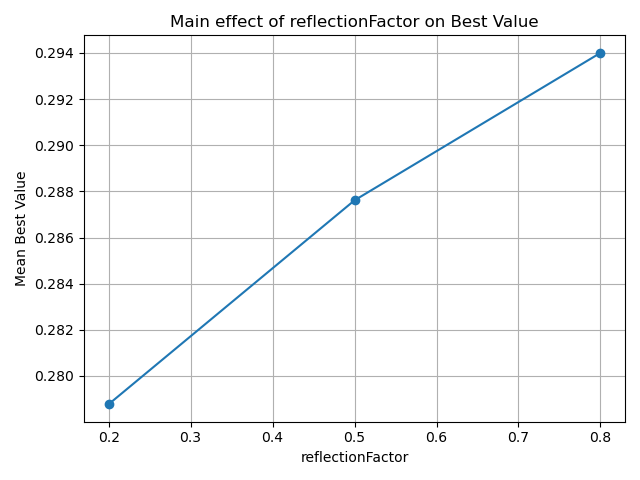
\includegraphics[scale=0.3]{fmsynth_reflectionFactor}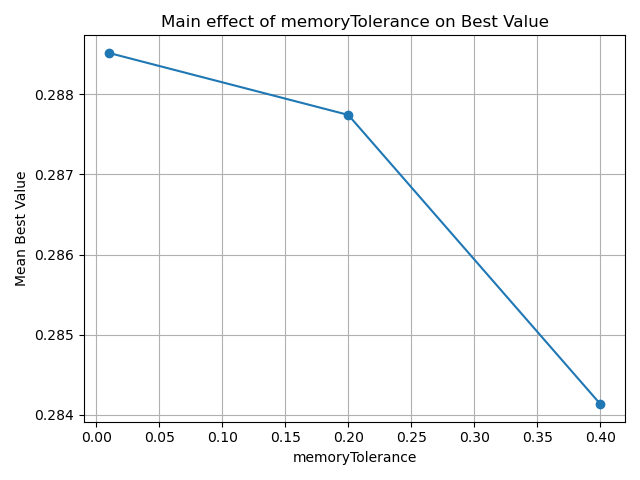
\includegraphics[scale=0.3]{fmsynth_memoryTolerance}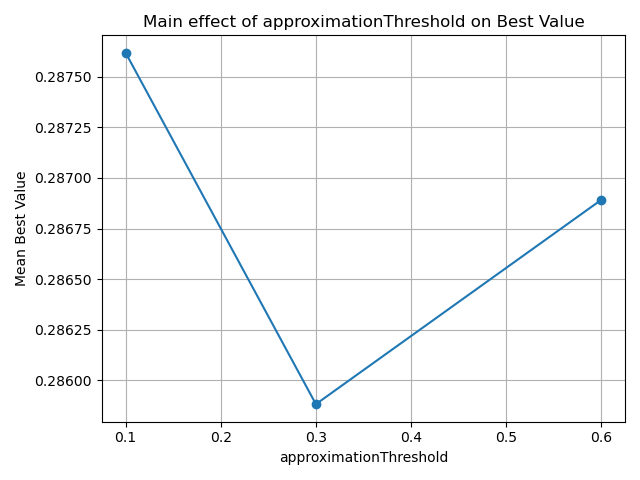
\includegraphics[scale=0.3]{fmsynth_approximationThreshold}

\caption{Graphical representation of Reflection factor, Memory Tolerance and
Approximation Threshold for the {\footnotesize\textbf{Frequency Modulated
Sound Waves}} problem\label{fig:fmsw}}
\end{figure}

\begin{table}[H]
\caption{Sensitivity analysis of the method parameters for the {\footnotesize\textbf{Lennard-Jones
Potential}} problem\label{tab:ljp}}

\centering{}{\footnotesize{}%
\begin{tabular}{|c|c|c|c|c|c|}
\hline 
\begin{cellvarwidth}[t]
\centering
{\footnotesize\textbf{Lennard Jones}}{\footnotesize\par}

{\footnotesize\textbf{Potential}}
\end{cellvarwidth} & {\footnotesize Value} & {\footnotesize Mean} & {\footnotesize Min} & {\footnotesize Max} & {\footnotesize Main range}\tabularnewline
\hline 
\hline 
\multirow{3}{*}{{\footnotesize Reflection Factor}} & {\footnotesize 0.2} & {\footnotesize -13.5131} & {\footnotesize -19.36124} & {\footnotesize -10.25016} & \multirow{3}{*}{{\footnotesize 3.03479}}\tabularnewline
\cline{2-5}
 & {\footnotesize 0.5} & {\footnotesize -12.83115} & {\footnotesize -19.61677} & {\footnotesize -8.00412} & \tabularnewline
\cline{2-5}
 & {\footnotesize 0.8} & {\footnotesize -10.47831} & {\footnotesize -17.01847} & {\footnotesize -6.01231} & \tabularnewline
\hline 
\multirow{3}{*}{{\footnotesize Memory Tolerance}} & {\footnotesize 0.01} & {\footnotesize -12.21917} & {\footnotesize -19.61677} & {\footnotesize -6.97152} & \multirow{3}{*}{{\footnotesize 0.08831}}\tabularnewline
\cline{2-5}
 & {\footnotesize 0.2} & {\footnotesize -12.29592} & {\footnotesize -19.36124} & {\footnotesize -6.21915} & \tabularnewline
\cline{2-5}
 & {\footnotesize 0.4} & {\footnotesize -12.30747} & {\footnotesize -18.87546} & {\footnotesize -6.01231} & \tabularnewline
\hline 
\multirow{3}{*}{{\footnotesize Approximation Threshold}} & {\footnotesize 0.1} & {\footnotesize -12.04052} & {\footnotesize -18.87546} & {\footnotesize -6.01231} & \multirow{3}{*}{{\footnotesize 0.40208}}\tabularnewline
\cline{2-5}
 & {\footnotesize 0.3} & {\footnotesize -12.33945} & {\footnotesize -17.36149} & {\footnotesize -6.64021} & \tabularnewline
\cline{2-5}
 & {\footnotesize 0.6} & {\footnotesize -12.44259} & {\footnotesize -19.61677} & {\footnotesize -6.21915} & \tabularnewline
\hline 
\end{tabular}}{\footnotesize\par}
\end{table}

\begin{figure}[H]
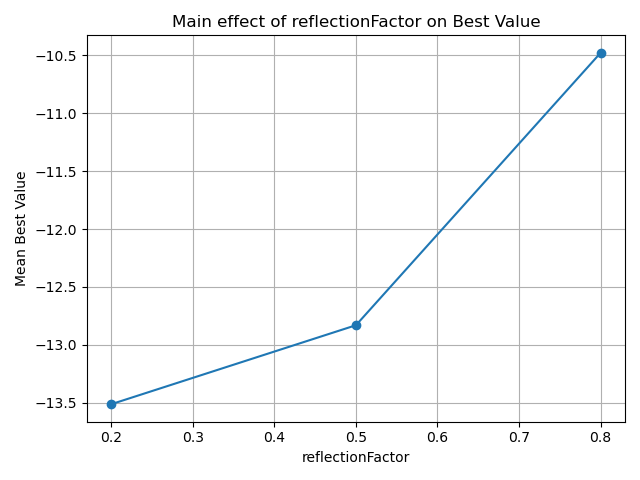
\includegraphics[scale=0.3]{lennardjones_reflectionFactor}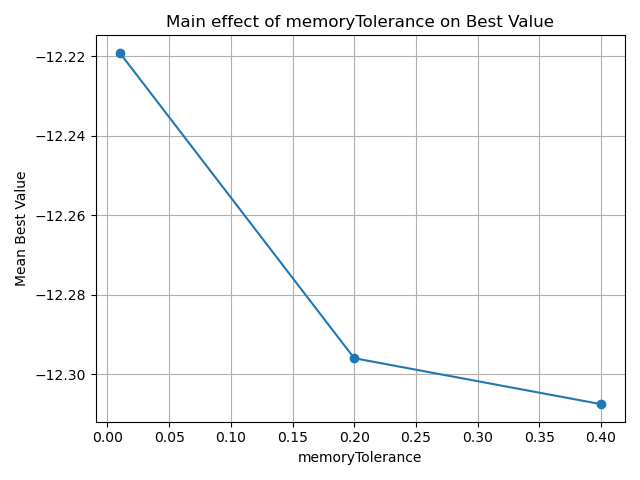
\includegraphics[scale=0.3]{lennardjones_memoryTolerane}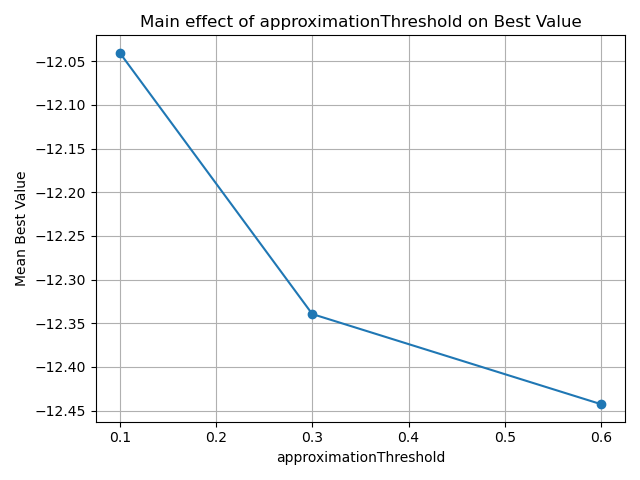
\includegraphics[scale=0.3]{lennardjones_approximationThreshold}

\caption{Graphical representation of Reflection factor, Memory Tolerance and
Approximation Threshold for the {\footnotesize\textbf{Lennard-Jones
Potential}} problem\label{fig:ljp}}
\end{figure}

\begin{table}[H]
\caption{Sensitivity analysis of the method parameters for the {\footnotesize\textbf{Dynamic
Economic Dispatch 1}} problem\label{tab:ded1}}

\centering{}{\footnotesize{}%
\begin{tabular}{|c|c|c|c|c|c|}
\hline 
\begin{cellvarwidth}[t]
\centering
{\footnotesize\textbf{Dynamic Economic}}{\footnotesize\par}

{\footnotesize\textbf{Dispatch 1}}
\end{cellvarwidth} & {\footnotesize Value} & {\footnotesize Mean} & {\footnotesize Min} & {\footnotesize Max} & {\footnotesize Main range}\tabularnewline
\hline 
\hline 
\multirow{3}{*}{{\footnotesize Reflection Factor}} & {\footnotesize 0.2} & {\footnotesize 498709776.79} & {\footnotesize 477135686.86} & {\footnotesize 525130205.59} & \multirow{3}{*}{{\footnotesize 13831927.78}}\tabularnewline
\cline{2-5}
 & {\footnotesize 0.5} & {\footnotesize 487372163.96} & {\footnotesize 463051832.53} & {\footnotesize 525005642.63} & \tabularnewline
\cline{2-5}
 & {\footnotesize 0.8} & {\footnotesize 484877849.01} & {\footnotesize 457195992.98} & {\footnotesize 523239555.02} & \tabularnewline
\hline 
\multirow{3}{*}{{\footnotesize Memory Tolerance}} & {\footnotesize 0.01} & {\footnotesize 490419307.37} & {\footnotesize 465337023.58} & {\footnotesize 525130205.59} & \multirow{3}{*}{{\footnotesize 175347.94}}\tabularnewline
\cline{2-5}
 & {\footnotesize 0.2} & {\footnotesize 490243959.43} & {\footnotesize 463051832.53} & {\footnotesize 525005642.63} & \tabularnewline
\cline{2-5}
 & {\footnotesize 0.4} & {\footnotesize 490296522.97} & {\footnotesize 457195992.98} & {\footnotesize 523251571.66} & \tabularnewline
\hline 
\multirow{3}{*}{{\footnotesize Approximation Threshold}} & {\footnotesize 0.1} & {\footnotesize 490754333.32} & {\footnotesize 465337023.58} & {\footnotesize 523251571.66} & \multirow{3}{*}{{\footnotesize 851763.73}}\tabularnewline
\cline{2-5}
 & {\footnotesize 0.3} & {\footnotesize 489902569.59} & {\footnotesize 457195992.98} & {\footnotesize 523611650.24} & \tabularnewline
\cline{2-5}
 & {\footnotesize 0.6} & {\footnotesize 490302886.86} & {\footnotesize 463051832.53} & {\footnotesize 525130205.59} & \tabularnewline
\hline 
\end{tabular}}{\footnotesize\par}
\end{table}

\begin{figure}[H]
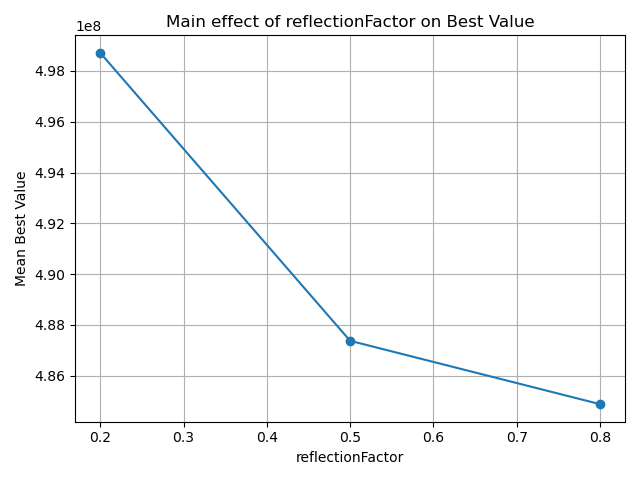
\includegraphics[scale=0.3]{ded1_reflectionFactor}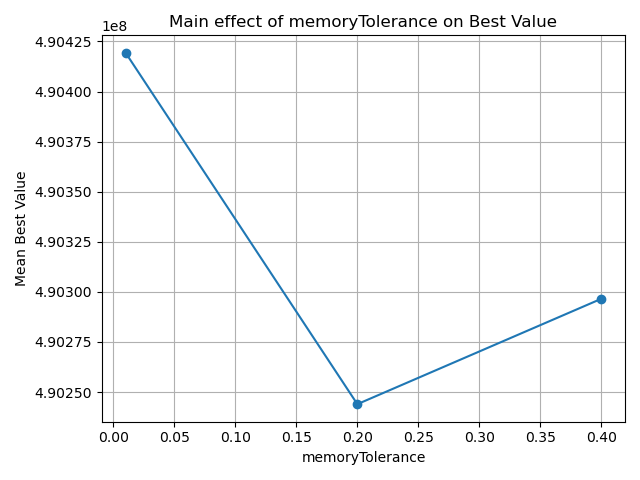
\includegraphics[scale=0.3]{ded1_memoryTolerance}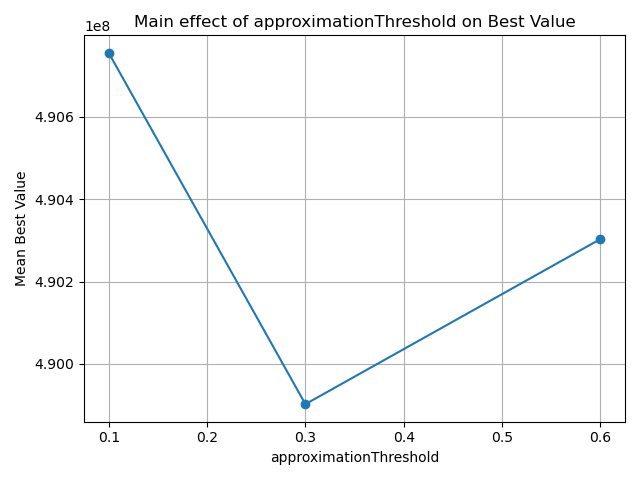
\includegraphics[scale=0.3]{ded1_approximationThreshold}

\caption{Graphical representation of Reflection factor, Memory Tolerance and
Approximation Threshold for the {\footnotesize\textbf{Dynamic Economic
Dispatch 1}} problem\label{fig:ded1}}
\end{figure}

\begin{table}[H]
\caption{Sensitivity analysis of the method parameters for the {\footnotesize\textbf{Static
Economic Load Dispatch 1}} problem\label{tab:eld1}}

\centering{}{\footnotesize{}%
\begin{tabular}{|c|c|c|c|c|c|}
\hline 
\begin{cellvarwidth}[t]
\centering
{\footnotesize\textbf{Static Economic}}{\footnotesize\par}

{\footnotesize\textbf{Load Dispatch 1}}
\end{cellvarwidth} & {\footnotesize Value} & {\footnotesize Mean} & {\footnotesize Min} & {\footnotesize Max} & {\footnotesize Main range}\tabularnewline
\hline 
\hline 
\multirow{3}{*}{{\footnotesize Reflection Factor}} & {\footnotesize 0.2} & {\footnotesize 7839.71673} & {\footnotesize 6487.28776} & {\footnotesize 51584.75127} & \multirow{3}{*}{{\footnotesize 5235.09}}\tabularnewline
\cline{2-5}
 & {\footnotesize 0.5} & {\footnotesize 13074.8164} & {\footnotesize 6557.19773} & {\footnotesize 713773.3893} & \tabularnewline
\cline{2-5}
 & {\footnotesize 0.8} & {\footnotesize 11316.61253} & {\footnotesize 6565.00778} & {\footnotesize 169504.9255} & \tabularnewline
\hline 
\multirow{3}{*}{{\footnotesize Memory Tolerance}} & {\footnotesize 0.01} & {\footnotesize 8716.80378} & {\footnotesize 6538.33345} & {\footnotesize 60471.06008} & \multirow{3}{*}{{\footnotesize 5531.27}}\tabularnewline
\cline{2-5}
 & {\footnotesize 0.2} & {\footnotesize 14248.08303} & {\footnotesize 6557.19773} & {\footnotesize 713773.3893} & \tabularnewline
\cline{2-5}
 & {\footnotesize 0.4} & {\footnotesize 9266.25885} & {\footnotesize 6487.28776} & {\footnotesize 111070.1477} & \tabularnewline
\hline 
\multirow{3}{*}{{\footnotesize Approximation Threshold}} & {\footnotesize 0.1} & {\footnotesize 10979.50246} & {\footnotesize 6487.28776} & {\footnotesize 355992.0461} & \multirow{3}{*}{{\footnotesize 3084.24}}\tabularnewline
\cline{2-5}
 & {\footnotesize 0.3} & {\footnotesize 9083.6991} & {\footnotesize 6569.6912} & {\footnotesize 79594.33844} & \tabularnewline
\cline{2-5}
 & {\footnotesize 0.6} & {\footnotesize 12167.9441} & {\footnotesize 6557.19773} & {\footnotesize 713773.3893} & \tabularnewline
\hline 
\end{tabular}}{\footnotesize\par}
\end{table}

\begin{figure}[H]
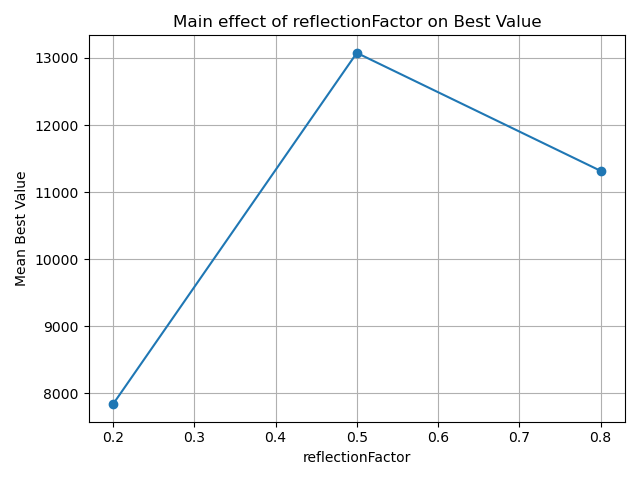
\includegraphics[scale=0.3]{eld_reflecctionFactor}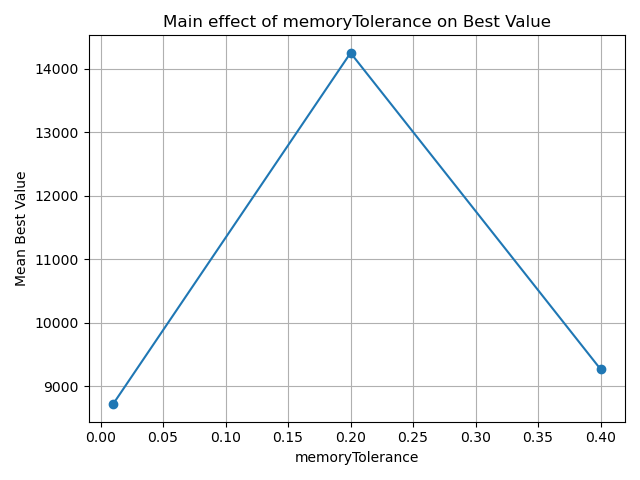
\includegraphics[scale=0.3]{eld_memoryTolerance}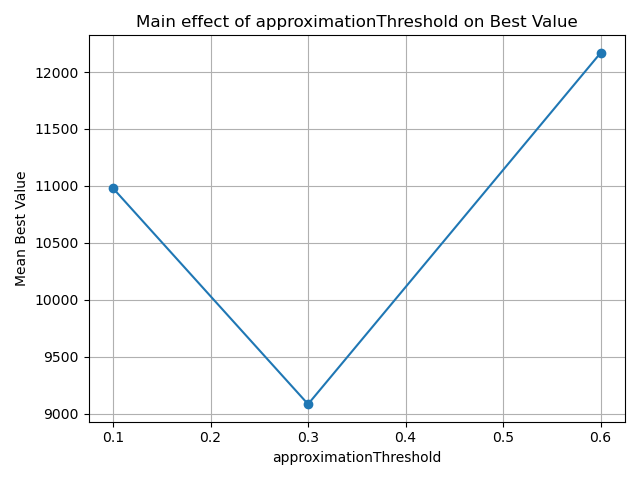
\includegraphics[scale=0.3]{eld_approximationThreshold}

\caption{Graphical representation of Reflection factor, Memory Tolerance and
Approximation Threshold for the {\footnotesize\textbf{Static Economic
Load Dispatch 1}} problem\label{fig:eld1}}
\end{figure}

For each problem, a series of tables \ref{tab:fmsw} - \ref{tab:eld1}
and Figures \ref{fig:fmsw} - \ref{fig:eld1}, with detailed results
for each parameter is presented. Each row of a table corresponds to
a specific tested value of the parameter. The columns display the
mean best value (Mean Best), the minimum value (Min), and the maximum
value (Max). The \textquotedbl Main range\textquotedbl{} indicator
summarizes the extent of the parameter’s impact on the algorithm’s
performance, calculated as the difference between the highest and
lowest mean values observed for that parameter.

The quantitative analysis of these indicators provides valuable insight
into which features of the method have the greatest impact on the
optimization process. For example, in the Lennard Jones Potential
problem, the parameter reflectionFactor has a main effect range of
3.03, indicating that changing this parameter results in significant
performance variation. Conversely, in cases where the main effect
range is very small (such as approximationThreshold in Frequency Modulated
Sound Waves with a value of 0.00174), the parameter exhibits low sensitivity,
which indicates that the method is stable with respect to changes
in this parameter. It is also noteworthy that parameter sensitivity
is not constant across problems. For instance, reflectionFactor has
moderate or negligible effect on Frequency Modulated Sound Waves,
but becomes a particularly important parameter for Lennard Jones Potential
and Static Economic Load Dispatch 1, as reflected in the corresponding
ranges. This behavior aligns with optimization theory, which states
that each problem has a “landscape” that interacts differently with
the exploration and exploitation mechanisms of each algorithm.

On the other hand, parameters such as memoryTolerance and approximationThreshold
often have lower main effect ranges. This can be interpreted as an
indication that the memory process and the evaluation approach are
relatively robust for this particular set of problems, and/or that
the selected values for these parameters do not differ enough to cause
substantial changes in performance.

Sensitivity analysis clearly highlights the parameters that should
be targeted during method optimization, while also indicating those
that can be set using general rules without significant risk of performance
loss. 

\subsection{Comparison of ECHO method with others\label{subsec:comparisonECHO}}

The analysis of the results presented in Tables \ref{tab:algorithmsBestAndMean},
\ref{tab:rankingBestAndMean}, and \ref{tab:finalRanking} was based
on a rigorously standardized experimental protocol to ensure the reliability
and comparability of the methods. Specifically, for Table \ref{tab:algorithmsBestAndMean},
the termination criterion was strictly set to a fixed number of function
evaluations (1,500,000), providing all methods with equal opportunities
for exploration in the solution space. For each method, the best value
(i.e., the lowest objective function value found) and the mean value
over 30 independent runs were recorded, thus capturing both the maximum
and average performance in a statistically substantiated manner. Subsequently,
in Table \ref{tab:rankingBestAndMean}, the methods were ranked for
each problem according to their performance, with 1 corresponding
to the best and 5 to the least effective performance among the five
methods. For drawing overall conclusions, Table \ref{tab:finalRanking}
presents the total sum of the ranks obtained by each method for both
the best and mean values, and this aggregate score was divided by
the total number of positions (i.e., the number of methods multiplied
by two, to account for both criteria), providing a composite measure
for comparing overall performance. Thus, the smallest average total
score indicates the most effective method, enabling an objective evaluation
of the comparative superiority of each approach across the full set
of problems.

{\tiny{}
\begin{sidewaystable}[H]
{\footnotesize\caption{Algorithms’ Comparison Based on Best and Mean after 1.5e+5 FEs\label{tab:algorithmsBestAndMean}}
}{\footnotesize\par}
\centering{}{\tiny{}%
\begin{tabular}{|V{\linewidth}|c|c|c|c|c|c|c|c|c|c|c|c|c|c|c|}
\hline 
{\tiny\textbf{Problem}} & \begin{cellvarwidth}[t]
\centering
{\tiny\textbf{CLPSO}}{\tiny{} \citep{Liang}}{\tiny\par}

{\tiny\textbf{Best}}
\end{cellvarwidth} & \begin{cellvarwidth}[t]
\centering
{\tiny\textbf{CLPSO}}{\tiny\par}

{\tiny\textbf{Mean}}
\end{cellvarwidth} & \begin{cellvarwidth}[t]
\centering
{\tiny CLPSO}{\tiny\par}

{\tiny SD}
\end{cellvarwidth} & \begin{cellvarwidth}[t]
\centering
{\tiny\textbf{SaDE }}{\tiny\citep{Qin}}{\tiny\par}

{\tiny\textbf{Best}}
\end{cellvarwidth} & \begin{cellvarwidth}[t]
\centering
{\tiny\textbf{SaDE}}{\tiny\par}

{\tiny\textbf{Mean}}
\end{cellvarwidth} & \begin{cellvarwidth}[t]
\centering
{\tiny SaDE}{\tiny\par}

{\tiny SD}
\end{cellvarwidth} & \begin{cellvarwidth}[t]
\centering
{\tiny\textbf{jDE }}{\tiny\citep{Brest}}{\tiny\par}

{\tiny\textbf{Best}}
\end{cellvarwidth} & \begin{cellvarwidth}[t]
\centering
{\tiny\textbf{jDE}}{\tiny\par}

{\tiny\textbf{Mean}}
\end{cellvarwidth} & \begin{cellvarwidth}[t]
\centering
{\tiny jDE}{\tiny\par}

{\tiny SD}
\end{cellvarwidth} & \begin{cellvarwidth}[t]
\centering
{\tiny\textbf{-ES}}{\tiny{} \citep{Hansen}}{\tiny\par}

{\tiny\textbf{Best}}
\end{cellvarwidth} & \begin{cellvarwidth}[t]
\centering
{\tiny\textbf{-ES}}{\tiny\par}

{\tiny\textbf{Mean}}
\end{cellvarwidth} & \begin{cellvarwidth}[t]
\centering
{\tiny -ES}{\tiny\par}

{\tiny SD}
\end{cellvarwidth} & \begin{cellvarwidth}[t]
\centering
{\tiny\textbf{EO}}{\tiny\par}

{\tiny\textbf{Best}}
\end{cellvarwidth} & \begin{cellvarwidth}[t]
\centering
{\tiny\textbf{EO}}{\tiny\par}

{\tiny\textbf{Mean}}
\end{cellvarwidth} & \begin{cellvarwidth}[t]
\centering
{\tiny EO}{\tiny\par}

{\tiny ST}
\end{cellvarwidth}\tabularnewline
\hline 
\hline 
{\tiny\textbf{Parameter Estimation}}{\tiny\par}

{\tiny\textbf{for Frequency}}{\tiny\par}

{\tiny\textbf{Modulated}}{\tiny\par}

{\tiny\textbf{Sound Waves}} & {\tiny 0.1314837477} & {\tiny 0.2124981688} & {\tiny 0.030223102} & {\tiny 0.1899428536} & {\tiny 0.2025566839} & {\tiny 0.009271896} & {\tiny 0.116157541} & {\tiny 0.146008756} & {\tiny 0.035009569} & {\tiny 0.18160915970} & {\tiny 0.256863966} & {\tiny 0.044727545} & {\tiny 0.242608779} & {\tiny 0.285913022} & {\tiny 0.022991904}\tabularnewline
\hline 
{\tiny\textbf{Lennard-Jones}}{\tiny\par}

{\tiny\textbf{Potential}} & {\tiny -13.43649135} & {\tiny -10.25073403} & {\tiny 1.02903617} & {\tiny -24.86870825} & {\tiny -22.6693403} & {\tiny 1.127265561} & {\tiny -29.98126575} & {\tiny -27.49258505} & {\tiny 1.235083397} & {\tiny -28.42253189} & {\tiny -25.78783328} & {\tiny 2.27119571} & {\tiny -15.82941908} & {\tiny -12.20055451} & {\tiny 1.743688768}\tabularnewline
\hline 
{\tiny\textbf{Bifunctional}}{\tiny\par}

{\tiny\textbf{CatalystBlend}}{\tiny\par}

{\tiny\textbf{Optimal Control}} & {\tiny -0.000286591} & {\tiny -0.000286591} & {\tiny 1.157726295e-16} & {\tiny -0.000286591} & {\tiny -0.000286591} & {\tiny 5.513684428e-20} & {\tiny -0.000286591} & {\tiny -0.000286591} & {\tiny 5.513684428e-20} & {\tiny -0.000286591} & {\tiny -0.000286591} & {\tiny 5.513684428e-20} & {\tiny -0.000286591} & {\tiny -0.000286591} & {\tiny 9.361236018e-11}\tabularnewline
\hline 
{\tiny\textbf{Optimal Control}}{\tiny\par}

{\tiny\textbf{of a Non-Linear}}{\tiny\par}

{\tiny\textbf{Stirred Tank Reactor}} & {\tiny 0.3903767228} & {\tiny 0.3903767228} & {\tiny 0} & {\tiny 0.3903767228} & {\tiny 0.3903767228} & {\tiny 0} & {\tiny 0.390376723} & {\tiny 0.390376723} & {\tiny 0} & {\tiny 0.3903767228} & {\tiny 0.390376723} & {\tiny 0} & {\tiny 0.3903767228} & {\tiny 0.390376723} & {\tiny 0}\tabularnewline
\hline 
{\tiny\textbf{Tersoff Potential}}{\tiny\par}

{\tiny\textbf{for model Si (B)}} & {\tiny -28.23544117} & {\tiny -26.18834522} & {\tiny 1.05654251} & {\tiny -3.107773136} & {\tiny 25.4711091} & {\tiny 16.7202543} & {\tiny -13.51157064} & {\tiny -3.983690794} & {\tiny 6.666047747} & {\tiny -29.26244222} & {\tiny -27.5889735} & {\tiny 1.040646284} & {\tiny -27.33646273} & {\tiny -24.93278552} & {\tiny 1.277547861}\tabularnewline
\hline 
{\tiny\textbf{Tersoff Potential}}{\tiny\par}

{\tiny\textbf{for model Si (C)}} & {\tiny -30.85200257} & {\tiny -28.87349048} & {\tiny 0.988024149} & {\tiny -11.60719468} & {\tiny 22.08963599} & {\tiny 18.5809093} & {\tiny -18.76214649} & {\tiny -8.506037168} & {\tiny 5.543190141} & {\tiny -33.19699356} & {\tiny -31.79270914} & {\tiny 0.828194234} & {\tiny -31.48064458} & {\tiny -28.96566368} & {\tiny 1.440816542}\tabularnewline
\hline 
{\tiny\textbf{Spread Spectrum}}{\tiny\par}

{\tiny\textbf{RadarPolly}}{\tiny\par}

{\tiny\textbf{phaseCode Design}} & {\tiny 1.085334991} & {\tiny 1.343956153} & {\tiny 0.148708837} & {\tiny 1.536501579} & {\tiny 2.150881715} & {\tiny 0.198607499} & {\tiny 1.525870558} & {\tiny 1.812042166} & {\tiny 0.171213339} & {\tiny 0.01} & {\tiny 0.171988666} & {\tiny 0.137892008} & {\tiny 0.446845407} & {\tiny 0.794854574} & {\tiny 0.206703444}\tabularnewline
\hline 
{\tiny\textbf{Transmission}}{\tiny\par}

{\tiny\textbf{Network}}{\tiny\par}

{\tiny\textbf{Expansion Planning}} & {\tiny 250} & {\tiny 250} & {\tiny 0} & {\tiny 250} & {\tiny 250} & {\tiny 0} & {\tiny 250} & {\tiny 250} & {\tiny 0} & {\tiny 250} & {\tiny 250} & {\tiny 0} & {\tiny 250} & {\tiny 250} & {\tiny 0}\tabularnewline
\hline 
{\tiny\textbf{Electricity}}{\tiny\par}

{\tiny\textbf{Transmission}}{\tiny\par}

{\tiny\textbf{Pricing}} & {\tiny 13,775,010.10} & {\tiny 13,775,395.07} & {\tiny 222.9723613} & {\tiny 23,481,009.86} & {\tiny 30,034,934.81} & {\tiny 3,264,767.4} & {\tiny 14,020,627.84} & {\tiny 14,820,953.78} & {\tiny 276,142.5345} & {\tiny 13,775,841.77} & {\tiny 13,787,550.18} & {\tiny 6136.744382} & {\tiny 13,775,640.18} & {\tiny 13,776,968.1} & {\tiny 481.2205121}\tabularnewline
\hline 
{\tiny\textbf{Circular Antenna}}{\tiny\par}

{\tiny\textbf{Array Design}} & {\tiny 0.006933401045} & {\tiny 0.05181551798} & {\tiny 0.070674314} & {\tiny 0.02142329927} & {\tiny 0.03892428051} & {\tiny 0.008183211} & {\tiny 0.006820072} & {\tiny 0.017657998} & {\tiny 0.022383475} & {\tiny 0.007204797576} & {\tiny 0.008635655364} & {\tiny 0.000917821} & {\tiny 0.019998298} & {\tiny 0.173367157} & {\tiny 0.079463074}\tabularnewline
\hline 
{\tiny\textbf{Dynamic Economic}}{\tiny\par}

{\tiny\textbf{Dispatch 1}} & {\tiny 428,607,927.60} & {\tiny 435,250,914.50} & {\tiny 2973190.125} & {\tiny 968,042,312.10} & {\tiny 1,034,679,775.00} & {\tiny 25,667,290.12} & {\tiny 968,042,312.1} & {\tiny 1,034,393,036} & {\tiny 25,445,935.78} & {\tiny 88,285.60} & {\tiny 102,776.71} & {\tiny 6688.08697} & {\tiny 464,634,158.9} & {\tiny 479,810,672.1} & {\tiny 10,428,912.68}\tabularnewline
\hline 
{\tiny\textbf{Dynamic Economic}}{\tiny\par}

{\tiny\textbf{Dispatch 2}} & {\tiny 33,031,590.31} & {\tiny 53,906,147.38} & {\tiny 8,492,239.111} & {\tiny 845,287,898.30} & {\tiny 913,715,793.20} & {\tiny 30,667,287.54} & {\tiny 340,091,475.3} & {\tiny 397,471,715.1} & {\tiny 37,259,947.14} & {\tiny 502,699.42} & {\tiny 577,720.15} & {\tiny 193,951.4891} & {\tiny 52,463,484.01} & {\tiny 73,536,820.82} & {\tiny 13625891.45}\tabularnewline
\hline 
{\tiny\textbf{Static Economic}}{\tiny\par}

{\tiny\textbf{Load Dispatch 1}} & {\tiny 6554.67} & {\tiny 7668.33} & {\tiny 1245.137667} & {\tiny 16,877.92} & {\tiny 101,588.39} & {\tiny 81,105.92078} & {\tiny 6163.749006} & {\tiny 6778.527028} & {\tiny 3004.59066} & {\tiny 6657.61} & {\tiny 415,917.46} & {\tiny 68,544.4983} & {\tiny 6603.922422} & {\tiny 10,413.46457} & {\tiny 7716.333599}\tabularnewline
\hline 
{\tiny\textbf{Static Economic}}{\tiny\par}

{\tiny\textbf{Load Dispatch 2}} & {\tiny 19,030.36} & {\tiny 20,699} & {\tiny 2922.047235} & {\tiny 2,600,565.21} & {\tiny 9,329,466.81} & {\tiny 4,019,053.284} & {\tiny 1,161,578.904} & {\tiny 3,671,587.605} & {\tiny 1,542,286.275} & {\tiny 763,001.22} & {\tiny 1,425,815.44} & {\tiny 377,126.8219} & {\tiny 19,338.19222} & {\tiny 35,064.4314} & {\tiny 19,829.76015}\tabularnewline
\hline 
{\tiny\textbf{Static Economic}}{\tiny\par}

{\tiny\textbf{Load Dispatch 3}} & {\tiny 470,192,288.30} & {\tiny 470,294,703.20} & {\tiny 57,822.41621} & {\tiny 478,069,615.30} & {\tiny 541,898,763.00} & {\tiny 20,128,777.18} & {\tiny 471,058,115.8} & {\tiny 471,963,142.3} & {\tiny 529,633.389} & {\tiny 470,023,232.30} & {\tiny 470,023,232.30} & {\tiny 1.848771369e-07} & {\tiny 470,350,624.6} & {\tiny 4,705,81625.1} & {\tiny 182,643.2251}\tabularnewline
\hline 
{\tiny\textbf{Static Economic}}{\tiny\par}

{\tiny\textbf{Load Dispatch 4}} & {\tiny 884,980.56} & {\tiny 1,423,887.36} & {\tiny 285,794.4518} & {\tiny 14,170,362.58} & {\tiny 106,749,078.50} & {\tiny 73,147,979.72} & {\tiny 6,482,592.714} & {\tiny 17,527,314.24} & {\tiny 5,306,489.46} & {\tiny 476,053.52} & {\tiny 2,925,852.94} & {\tiny 1,268,161.817} & {\tiny 138,516.9427} & {\tiny 331,608.7229} & {\tiny 125,778.3196}\tabularnewline
\hline 
{\tiny\textbf{Static Economic}}{\tiny\par}

{\tiny\textbf{Load Dispatch 5}} & {\tiny 8,105,947,615.00} & {\tiny 8,110,924,071.00} & {\tiny 4,422,895.726} & {\tiny 1.312720405e+10} & {\tiny 1.354375465e+10} & {\tiny 213,865,059.7} & {\tiny 8,453,090,778} & {\tiny 8,459,337,082} & {\tiny 2,874,979.192} & {\tiny 8,072,077,963.00} & {\tiny 8,084,017,791.00} & {\tiny 4,623,617.36} & {\tiny 8,076,264,799} & {\tiny 8,295,168,707} & {\tiny 193,563,112.7}\tabularnewline
\hline 
\end{tabular}}{\tiny\par}
\end{sidewaystable}
}
\begin{sidewaystable}[H]
\caption{Detailed Ranking of Algorithms Based on Best and Mean after 1.5e+5
FEs\label{tab:rankingBestAndMean}}

\centering{}{\footnotesize{}%
\begin{tabular}{|V{\linewidth}|c|c|c|c|c|c|c|c|c|c|}
\hline 
{\footnotesize\textbf{Problem}} & \begin{cellvarwidth}[t]
\centering
{\footnotesize\textbf{CLPSO}}{\footnotesize\par}

{\footnotesize\textbf{best}}
\end{cellvarwidth} & \begin{cellvarwidth}[t]
\centering
{\footnotesize\textbf{CLPSO}}{\footnotesize\par}

{\footnotesize\textbf{Mean}}
\end{cellvarwidth} & \begin{cellvarwidth}[t]
\centering
{\footnotesize\textbf{SaDE}}{\footnotesize\par}

{\footnotesize\textbf{best}}
\end{cellvarwidth} & \begin{cellvarwidth}[t]
\centering
{\footnotesize\textbf{SaDE}}{\footnotesize\par}

{\footnotesize\textbf{Mean}}
\end{cellvarwidth} & \begin{cellvarwidth}[t]
\centering
{\footnotesize\textbf{jDE}}{\footnotesize\par}

{\footnotesize\textbf{Best}}
\end{cellvarwidth} & \begin{cellvarwidth}[t]
\centering
{\footnotesize\textbf{jDE}}{\footnotesize\par}

{\footnotesize\textbf{Mean}}
\end{cellvarwidth} & \begin{cellvarwidth}[t]
\centering
{\footnotesize\textbf{-ES}}{\footnotesize\par}

{\footnotesize\textbf{best}}
\end{cellvarwidth} & \begin{cellvarwidth}[t]
\centering
{\footnotesize\textbf{-ES}}{\footnotesize\par}

{\footnotesize\textbf{Mean}}
\end{cellvarwidth} & \begin{cellvarwidth}[t]
\centering
{\footnotesize\textbf{EO}}{\footnotesize\par}

{\footnotesize\textbf{Best}}
\end{cellvarwidth} & \begin{cellvarwidth}[t]
\centering
{\footnotesize\textbf{EO}}{\footnotesize\par}

{\footnotesize\textbf{Mean}}
\end{cellvarwidth}\tabularnewline
\hline 
\hline 
{\footnotesize\textbf{Parameter Estimation for}}{\footnotesize\par}

{\footnotesize\textbf{Frequency-Modulated Sound Waves}} & {\footnotesize 2} & {\footnotesize 3} & {\footnotesize 4} & {\footnotesize 2} & {\footnotesize 1} & {\footnotesize 1} & {\footnotesize 3} & {\footnotesize 4} & {\footnotesize 5} & {\footnotesize 5}\tabularnewline
\hline 
{\footnotesize\textbf{Lennard-Jones}}{\footnotesize\par}

{\footnotesize\textbf{Potential}} & {\footnotesize 5} & {\footnotesize 5} & {\footnotesize 3} & {\footnotesize 3} & {\footnotesize 2} & {\footnotesize 2} & {\footnotesize 1} & {\footnotesize 1} & {\footnotesize 4} & {\footnotesize 4}\tabularnewline
\hline 
{\footnotesize\textbf{BifunctionalCatalyst Blend}}{\footnotesize\par}

{\footnotesize\textbf{Optimal Control}} & {\footnotesize 1} & {\footnotesize 1} & {\footnotesize 1} & {\footnotesize 1} & {\footnotesize 1} & {\footnotesize 1} & {\footnotesize 1} & {\footnotesize 1} & {\footnotesize 1} & {\footnotesize 1}\tabularnewline
\hline 
{\footnotesize\textbf{Optimal Control of a}}{\footnotesize\par}

{\footnotesize\textbf{Non-Linear Stirred}}{\footnotesize\par}

{\footnotesize\textbf{Tank Reactor}} & {\footnotesize 1} & {\footnotesize 1} & {\footnotesize 1} & {\footnotesize 1} & {\footnotesize 1} & {\footnotesize 1} & {\footnotesize 1} & {\footnotesize 1} & {\footnotesize 1} & {\footnotesize 1}\tabularnewline
\hline 
{\footnotesize\textbf{Tersoff Potential}}{\footnotesize\par}

{\footnotesize\textbf{for model Si (B)}} & {\footnotesize 2} & {\footnotesize 2} & {\footnotesize 5} & {\footnotesize 5} & {\footnotesize 4} & {\footnotesize 4} & {\footnotesize 1} & {\footnotesize 1} & {\footnotesize 3} & {\footnotesize 3}\tabularnewline
\hline 
{\footnotesize\textbf{Tersoff Potential}}{\footnotesize\par}

{\footnotesize\textbf{for model Si (C)}} & {\footnotesize 3} & {\footnotesize 3} & {\footnotesize 5} & {\footnotesize 5} & {\footnotesize 4} & {\footnotesize 4} & {\footnotesize 1} & {\footnotesize 1} & {\footnotesize 2} & {\footnotesize 2}\tabularnewline
\hline 
{\footnotesize\textbf{Spread Spectrum Radar}}{\footnotesize\par}

{\footnotesize\textbf{Polly phaseCode Design}} & {\footnotesize 3} & {\footnotesize 3} & {\footnotesize 5} & {\footnotesize 5} & {\footnotesize 4} & {\footnotesize 4} & {\footnotesize 1} & {\footnotesize 1} & {\footnotesize 2} & {\footnotesize 2}\tabularnewline
\hline 
{\footnotesize\textbf{Transmission Network}}{\footnotesize\par}

{\footnotesize\textbf{Expansion Planning}} & {\footnotesize 1} & {\footnotesize 1} & {\footnotesize 1} & {\footnotesize 1} & {\footnotesize 1} & {\footnotesize 1} & {\footnotesize 1} & {\footnotesize 1} & {\footnotesize 1} & {\footnotesize 1}\tabularnewline
\hline 
{\footnotesize\textbf{Electricity Transmission}}{\footnotesize\par}

{\footnotesize\textbf{Pricing}} & {\footnotesize 1} & {\footnotesize 1} & {\footnotesize 5} & {\footnotesize 5} & {\footnotesize 4} & {\footnotesize 4} & {\footnotesize 3} & {\footnotesize 3} & {\footnotesize 2} & {\footnotesize 2}\tabularnewline
\hline 
{\footnotesize\textbf{Circular Antenna}}{\footnotesize\par}

{\footnotesize\textbf{Array Design}} & {\footnotesize 2} & {\footnotesize 4} & {\footnotesize 5} & {\footnotesize 3} & {\footnotesize 1} & {\footnotesize 2} & {\footnotesize 3} & {\footnotesize 1} & {\footnotesize 4} & {\footnotesize 5}\tabularnewline
\hline 
{\footnotesize\textbf{Dynamic Economic}}{\footnotesize\par}

{\footnotesize\textbf{Dispatch 1}} & {\footnotesize 2} & {\footnotesize 2} & {\footnotesize 4} & {\footnotesize 5} & {\footnotesize 5} & {\footnotesize 4} & {\footnotesize 1} & {\footnotesize 1} & {\footnotesize 3} & {\footnotesize 3}\tabularnewline
\hline 
{\footnotesize\textbf{Dynamic Economic}}{\footnotesize\par}

{\footnotesize\textbf{Dispatch 2}} & {\footnotesize 2} & {\footnotesize 2} & {\footnotesize 5} & {\footnotesize 5} & {\footnotesize 3} & {\footnotesize 4} & {\footnotesize 1} & {\footnotesize 1} & {\footnotesize 4} & {\footnotesize 3}\tabularnewline
\hline 
{\footnotesize\textbf{Static Economic}}{\footnotesize\par}

{\footnotesize\textbf{Load Dispatch 1}} & {\footnotesize 2} & {\footnotesize 2} & {\footnotesize 5} & {\footnotesize 5} & {\footnotesize 1} & {\footnotesize 1} & {\footnotesize 4} & {\footnotesize 4} & {\footnotesize 3} & {\footnotesize 3}\tabularnewline
\hline 
{\footnotesize\textbf{Static Economic}}{\footnotesize\par}

{\footnotesize\textbf{Load Dispatch 2}} & {\footnotesize 1} & {\footnotesize 1} & {\footnotesize 5} & {\footnotesize 5} & {\footnotesize 4} & {\footnotesize 4} & {\footnotesize 3} & {\footnotesize 3} & {\footnotesize 2} & {\footnotesize 2}\tabularnewline
\hline 
{\footnotesize\textbf{Static Economic}}{\footnotesize\par}

{\footnotesize\textbf{Load Dispatch 3}} & {\footnotesize 2} & {\footnotesize 2} & {\footnotesize 5} & {\footnotesize 5} & {\footnotesize 4} & {\footnotesize 4} & {\footnotesize 1} & {\footnotesize 1} & {\footnotesize 3} & {\footnotesize 3}\tabularnewline
\hline 
{\footnotesize\textbf{Static Economic}}{\footnotesize\par}

{\footnotesize\textbf{Load Dispatch 4}} & {\footnotesize 3} & {\footnotesize 3} & {\footnotesize 5} & {\footnotesize 5} & {\footnotesize 4} & {\footnotesize 4} & {\footnotesize 2} & {\footnotesize 2} & {\footnotesize 1} & {\footnotesize 1}\tabularnewline
\hline 
{\footnotesize\textbf{Static Economic}}{\footnotesize\par}

{\footnotesize\textbf{Load Dispatch 5}} & {\footnotesize 3} & {\footnotesize 2} & {\footnotesize 5} & {\footnotesize 5} & {\footnotesize 4} & {\footnotesize 4} & {\footnotesize 1} & {\footnotesize 1} & {\footnotesize 2} & {\footnotesize 3}\tabularnewline
\hline 
{\footnotesize\textbf{TOTAL}} & {\footnotesize\textbf{36}} & {\footnotesize\textbf{38}} & {\footnotesize\textbf{69}} & {\footnotesize\textbf{66}} & {\footnotesize\textbf{48}} & {\footnotesize\textbf{49}} & {\footnotesize\textbf{29}} & {\footnotesize\textbf{28}} & {\footnotesize\textbf{43}} & {\footnotesize\textbf{44}}\tabularnewline
\hline 
\end{tabular}}{\footnotesize\par}
\end{sidewaystable}
\begin{table}[H]
\caption{Comparison of Algorithms and Final Ranking\label{tab:finalRanking}}

\centering{}%
\begin{tabular}{|c|c|c|c|c|c|}
\hline 
\textbf{Problem} & \textbf{Best} & \textbf{Mean} & \textbf{Overall} & \textbf{Average} & \textbf{Rang}\tabularnewline
\hline 
\hline 
\textbf{-ES} & 29 & 28 & 57 & 1.5833 & \textbf{1}\tabularnewline
\hline 
\textbf{CLPSO} & 36 & 38 & 74 & 2.0555 & \textbf{2}\tabularnewline
\hline 
\textbf{EO} & 43 & 44 & 87 & 2.4166 & \textbf{3}\tabularnewline
\hline 
\textbf{jDE} & 48 & 49 & 97 & 2.6944 & \textbf{4}\tabularnewline
\hline 
\textbf{SaDE} & 69 & 66 & 135 & 3.75 & \textbf{5}\tabularnewline
\hline 
\end{tabular}
\end{table}

In the comparative assessment conducted in this subsection, the basic
form of the EO was benchmarked against other modern and internationally
recognized evolutionary algorithms such as SaDE, jDE, CLPSO, and CMA-ES,
which serve as the state-of-the-art reference for real-world global
optimization problems. The selection of these algorithms ensures a
fair and realistic comparison, as all are noted for their stability
and proven effectiveness in a wide range of practical applications
and complex problems, as also reflected in the CEC2011 benchmark.
The EO was implemented in its pure form, without the use of additional
memory or surrogate evaluation mechanisms, thus highlighting the intrinsic
ability of the method to address high-dimensional and complex problems
transparently.

The analysis of the results indicates that EO remains highly competitive
compared to the other examined methods across a substantial portion
of the tested problems. It achieves comparable best and mean values,
while exhibiting reduced variability between independent runs a feature
that reflects its stable performance and reliability in real-world
applications. Although in certain cases small deviations appear in
favor of competing algorithms, particularly in highly specialized
problem landscapes or in regions where intensive local exploitation
is advantageous, the overall findings confirm the robustness and effectiveness
of EO. The uniform use of a fixed population size (100 samples, except
for CMA-ES), identical stopping criteria and parameters (as specified
in Table 1), ensure absolute objectivity and fairness in the evaluation
framework.

Consequently, EO proves to be a highly promising alternative among
contemporary global optimization algorithms, highlighting its potential
for future development and adoption in real-world applications, where
the balance between speed, reliability, and implementation simplicity
remains a core requirement.

\subsection{The Echo method and neural networks\label{subsec:NNC}}

An additional experiment was conducted, where the ECHO+APP+MEM method
was used to train artificial neural networks \citep{nn1,nn2}, by
minimizing the so - called training error defined as:
\begin{equation}
E\left(N\left(\overrightarrow{x},\overrightarrow{w}\right)\right)=\sum_{i=1}^{M}\left(N\left(\overrightarrow{x}_{i},\overrightarrow{w}\right)-y_{i}\right)^{2}\label{eq:eq1}
\end{equation}
In this equation the function $N\left(\overrightarrow{x},\overrightarrow{w}\right)$
represents the artificial neural network which is applied on a vector
$\overrightarrow{x}$ and the vector $\overrightarrow{w}$ denotes
the parameter vector of the neural network. The set $\left(\overrightarrow{x_{i}},y_{i}\right),\ i=1,...,M$
represents the training set of the objective problem and the values
$y_{i}$ are the expected outputs for each pattern $\overrightarrow{x_{i}}$. 

To validate the ECHO+APP+MEM method, an extensive collection of classification
datasets was employed, sourced from various publicly available online
repositories. These datasets were obtained from:
\begin{enumerate}
\item The UCI database, \url{https://archive.ics.uci.edu/}(accessed on
5 July 2025)\citep{uci}
\item The Keel website, \url{https://sci2s.ugr.es/keel/datasets.php}(accessed
on 5 July2025)\citep{Keel}.
\item The Statlib URL \url{https://lib.stat.cmu.edu/datasets/index}(accessed
on 5 July 2025). 
\end{enumerate}
The experiments were conducted using the following datasets:
\begin{enumerate}
\item \textbf{Appendictis} which is a medical dataset \citep{appendicitis}. 
\item \textbf{Alcohol}, which is dataset regarding alcohol consumption \citep{alcohol}. 
\item \textbf{Australian}, which is a dataset produced from various bank
transactions \citep{australian}.
\item \textbf{Balance} dataset \citep{balance}, produced from various psychological
experiments.
\item \textbf{Circular} dataset, which is an artificial dataset.
\item \textbf{Cleveland}, a medical dataset which was discussed in a series
of papers \citep{cleveland1,cleveland2}. 
\item \textbf{Dermatology}, a medical dataset for dermatology problems \citep{dermatology}.
\item \textbf{Ecoli}, which is related to protein problems \citep{ecoli}.
\item \textbf{Glass} dataset, that contains measurements from glass component
analysis.
\item \textbf{Haberman}, a medical dataset related to breast cancer.
\item \textbf{Hayes-roth} dataset \citep{hayes-roth}.
\item \textbf{Heart}, which is a dataset related to heart diseases \citep{heart}.
\item \textbf{HeartAttack}, which is a medical dataset for the detection
of heart diseases
\item \textbf{Housevotes}, a dataset which is related to the Congressional
voting in USA \citep{housevotes}.
\item \textbf{Ionosphere}, a dataset that contains measurements from the
ionosphere \citep{ion1,ion2}.
\item \textbf{Liverdisorder}, a medical dataset that was studied thoroughly
in a series of papers\citep{liver,liver1}.
\item \textbf{Lymography} \citep{lymography}.
\item \textbf{Mammographic}, which is a medical dataset used for the prediction
of breast cancer \citep{mammographic}.
\item \textbf{Parkinsons}, which is a medical dataset used for the detection
of Parkinson's disease \citep{parkinsons1,parkinsons2}.
\item \textbf{Pima}, which is a medical dataset for the detection of diabetes\citep{pima}.
\item \textbf{Popfailures}, a dataset related to experiments regarding climate
\citep{popfailures}.
\item \textbf{Regions2}, a medical dataset applied to liver problems \citep{regions2}.
\item \textbf{Saheart}, which is a medical dataset concerning heart diseases\citep{saheart}.
\item \textbf{Segment} dataset \citep{segment}.
\item The \textbf{Sonar} dataset, related to sonar signals \citep{sonar}.
\item \textbf{Statheart}, a medical dataset related to heart diseases.
\item \textbf{Student}, which is a dataset regarding experiments in schools
\citep{student}.
\item \textbf{Transfusion}, which is a medical dataset \citep{transfusion}.
\item \textbf{Wdbc}, which is a medical dataset regarding breast cancer
\citep{wdbc1,wdbc2}.
\item \textbf{Wine}, a dataset regarding measurements about the quality
of wines \citep{wine1,wine2}.
\item \textbf{EEG}, which is dataset regardingEEG recordings \citep{eeg1,eeg2}.
From this dataset the following cases were used: Z\_F\_S, ZO\_NF\_S,
and ZONF\_S.
\item \textbf{Zoo}, which is a dataset regarding animal classification \citep{zoo}
.
\end{enumerate}
\begin{table}[H]
\begin{centering}
{\footnotesize{}%
\begin{tabular}{|l|c|c|c|c|c|}
\hline 
{\footnotesize\textbf{DATASET}} & {\footnotesize\textbf{GENETIC}} & {\footnotesize\textbf{ECHO}} & {\footnotesize\textbf{ECHO+APP}} & {\footnotesize\textbf{ECHO+MEM}} & {\footnotesize\textbf{ECHO+APP+MEM}}\tabularnewline
\hline 
\hline 
{\footnotesize\textbf{Appendicitis}} & {\footnotesize 18.10\%} & {\footnotesize 22.07\%} & {\footnotesize 22.47\%} & {\footnotesize 22.60\%} & {\footnotesize 22.77\%}\tabularnewline
\hline 
{\footnotesize\textbf{Alcohol}} & {\footnotesize 39.57\%} & {\footnotesize 18.91\%} & {\footnotesize 17.24\%} & {\footnotesize 17.77\%} & {\footnotesize 16.96\%}\tabularnewline
\hline 
{\footnotesize\textbf{Australian}} & {\footnotesize 32.10\%} & {\footnotesize 22.34\%} & {\footnotesize 22.34\%} & {\footnotesize 22.91\%} & {\footnotesize 23.16\%}\tabularnewline
\hline 
{\footnotesize\textbf{Balance}} & {\footnotesize 8.97\%} & {\footnotesize 7.10\%} & {\footnotesize 7.10\%} & {\footnotesize 7.22\%} & {\footnotesize 7.23\%}\tabularnewline
\hline 
{\footnotesize\textbf{Circular}} & {\footnotesize 5.99\%} & {\footnotesize 4.48\%} & {\footnotesize 4.48\%} & {\footnotesize 4.37\%} & {\footnotesize 4.37\%}\tabularnewline
\hline 
{\footnotesize\textbf{Cleveland}} & {\footnotesize 51.60\%} & {\footnotesize 45.74\%} & {\footnotesize 45.74\%} & {\footnotesize 46.60\%} & {\footnotesize 46.60\%}\tabularnewline
\hline 
{\footnotesize\textbf{Dermatology}} & {\footnotesize 30.58\%} & {\footnotesize 9.34\%} & {\footnotesize 9.34\%} & {\footnotesize 11.51\%} & {\footnotesize 11.51\%}\tabularnewline
\hline 
{\footnotesize\textbf{Ecoli}} & {\footnotesize 54.67\%} & {\footnotesize 45.89\%} & {\footnotesize 45.89\%} & {\footnotesize 48.94\%} & {\footnotesize 48.94\%}\tabularnewline
\hline 
{\footnotesize\textbf{Fert}} & {\footnotesize 28.50\%} & {\footnotesize 24.40\%} & {\footnotesize 24.13\%} & {\footnotesize 26.50\%} & {\footnotesize 24.57\%}\tabularnewline
\hline 
{\footnotesize\textbf{Glass}} & {\footnotesize 58.30\%} & {\footnotesize 50.24\%} & {\footnotesize 50.24\%} & {\footnotesize 49.43\%} & {\footnotesize 49.22\%}\tabularnewline
\hline 
{\footnotesize\textbf{Haberman}} & {\footnotesize 28.66\%} & {\footnotesize 28.71\%} & {\footnotesize 28.71\%} & {\footnotesize 28.80\%} & {\footnotesize 28.80\%}\tabularnewline
\hline 
{\footnotesize\textbf{Hayes-roth}} & {\footnotesize 56.18\%} & {\footnotesize 35.21\%} & {\footnotesize 35.21\%} & {\footnotesize 37.46\%} & {\footnotesize 37.46\%}\tabularnewline
\hline 
{\footnotesize\textbf{Heart}} & {\footnotesize 28.34\%} & {\footnotesize 18.10\%} & {\footnotesize 18.10\%} & {\footnotesize 19.00\%} & {\footnotesize 19.02\%}\tabularnewline
\hline 
{\footnotesize\textbf{HeartAttack}} & {\footnotesize 29.03\%} & {\footnotesize 20.06\%} & {\footnotesize 20.06\%} & {\footnotesize 20.15\%} & {\footnotesize 20.15\%}\tabularnewline
\hline 
{\footnotesize\textbf{Housevotes}} & {\footnotesize 6.62\%} & {\footnotesize 7.58\%} & {\footnotesize 7.68\%} & {\footnotesize 7.20\%} & {\footnotesize 7.10\%}\tabularnewline
\hline 
{\footnotesize\textbf{Ionosphere}} & {\footnotesize 15.14\%} & {\footnotesize 14.53\%} & {\footnotesize 14.53\%} & {\footnotesize 15.03\%} & {\footnotesize 15.08\%}\tabularnewline
\hline 
{\footnotesize\textbf{Liverdisorder}} & {\footnotesize 31.11\%} & {\footnotesize 31.82\%} & {\footnotesize 31.82\%} & {\footnotesize 32.48\%} & {\footnotesize 32.48\%}\tabularnewline
\hline 
{\footnotesize\textbf{LYMOGRAPHY}} & {\footnotesize 28.42\%} & {\footnotesize 24.60\%} & {\footnotesize 24.60\%} & {\footnotesize 26.02\%} & {\footnotesize 25.31\%}\tabularnewline
\hline 
{\footnotesize\textbf{Mammographic}} & {\footnotesize 19.88\%} & {\footnotesize 17.44\%} & {\footnotesize 17.45\%} & {\footnotesize 17.36\%} & {\footnotesize 17.36\%}\tabularnewline
\hline 
{\footnotesize\textbf{Parkinsons}} & {\footnotesize 18.05\%} & {\footnotesize 15.04\%} & {\footnotesize 14.95\%} & {\footnotesize 15.74\%} & {\footnotesize 15.21\%}\tabularnewline
\hline 
{\footnotesize\textbf{Pima}} & {\footnotesize 32.19\%} & {\footnotesize 26.34\%} & {\footnotesize 26.34\%} & {\footnotesize 26.78\%} & {\footnotesize 26.78\%}\tabularnewline
\hline 
{\footnotesize\textbf{Popfailures}} & {\footnotesize 5.94\%} & {\footnotesize 6.88\%} & {\footnotesize 6.88\%} & {\footnotesize 6.84\%} & {\footnotesize 6.84\%}\tabularnewline
\hline 
{\footnotesize\textbf{Regions2}} & {\footnotesize 29.39\%} & {\footnotesize 28.21\%} & {\footnotesize 28.21\%} & {\footnotesize 30.07\%} & {\footnotesize 30.12\%}\tabularnewline
\hline 
{\footnotesize\textbf{Saheart}} & {\footnotesize 34.86\%} & {\footnotesize 32.71\%} & {\footnotesize 32.91\%} & {\footnotesize 32.46\%} & {\footnotesize 32.46\%}\tabularnewline
\hline 
{\footnotesize\textbf{Segment}} & {\footnotesize 57.72\%} & {\footnotesize 14.82\%} & {\footnotesize 14.82\%} & {\footnotesize 16.91\%} & {\footnotesize 16.87\%}\tabularnewline
\hline 
{\footnotesize\textbf{Sonar}} & {\footnotesize 22.40\%} & {\footnotesize 19.98\%} & {\footnotesize 20.52\%} & {\footnotesize 20.37\%} & {\footnotesize 20.07\%}\tabularnewline
\hline 
{\footnotesize\textbf{Spiral}} & {\footnotesize 48.66\%} & {\footnotesize 41.91\%} & {\footnotesize 41.91\%} & {\footnotesize 42.24\%} & {\footnotesize 42.24\%}\tabularnewline
\hline 
{\footnotesize\textbf{STATHEART}} & {\footnotesize 27.25\%} & {\footnotesize 19.45\%} & {\footnotesize 19.45\%} & {\footnotesize 20.24\%} & {\footnotesize 20.24\%}\tabularnewline
\hline 
{\footnotesize\textbf{Student}} & {\footnotesize 5.61\%} & {\footnotesize 5.84\%} & {\footnotesize 5.84\%} & {\footnotesize 5.98\%} & {\footnotesize 5.98\%}\tabularnewline
\hline 
{\footnotesize\textbf{Transfusion}} & {\footnotesize 24.87\%} & {\footnotesize 23.70\%} & {\footnotesize 23.70\%} & {\footnotesize 24.09\%} & {\footnotesize 24.09\%}\tabularnewline
\hline 
{\footnotesize\textbf{Wdbc}} & {\footnotesize 8.56\%} & {\footnotesize 3.92\%} & {\footnotesize 3.92\%} & {\footnotesize 4.72\%} & {\footnotesize 4.60\%}\tabularnewline
\hline 
{\footnotesize\textbf{Wine}} & {\footnotesize 19.20\%} & {\footnotesize 10.45\%} & {\footnotesize 10.45\%} & {\footnotesize 12.84\%} & {\footnotesize 13.88\%}\tabularnewline
\hline 
{\footnotesize\textbf{Z\_F\_S}} & {\footnotesize 10.73\%} & {\footnotesize 8.48\%} & {\footnotesize 8.48\%} & {\footnotesize 8.71\%} & {\footnotesize 7.89\%}\tabularnewline
\hline 
{\footnotesize\textbf{ZO\_NF\_S}} & {\footnotesize 21.54\%} & {\footnotesize 5.15\%} & {\footnotesize 5.15\%} & {\footnotesize 5.61\%} & {\footnotesize 5.99\%}\tabularnewline
\hline 
{\footnotesize\textbf{ZONF\_S}} & {\footnotesize 4.36\%} & {\footnotesize 2.96\%} & {\footnotesize 2.96\%} & {\footnotesize 2.91\%} & {\footnotesize 2.83\%}\tabularnewline
\hline 
{\footnotesize\textbf{ZOO}} & {\footnotesize 9.50\%} & {\footnotesize 3.60\%} & {\footnotesize 3.60\%} & {\footnotesize 3.60\%} & {\footnotesize 3.70\%}\tabularnewline
\hline 
{\footnotesize\textbf{AVERAGE}} & {\footnotesize\textbf{26.46\%}} & {\footnotesize\textbf{19.94\%}} & {\footnotesize\textbf{19.92\%}} & {\footnotesize\textbf{20.60\%}} & {\footnotesize\textbf{20.50\%}}\tabularnewline
\hline 
\end{tabular}}{\footnotesize\par}
\par\end{centering}
\caption{Comparative Classification Error Rates Across Datasets Using ECHO-Based
and Genetic Optimization Methods\label{tab:mlp}}
\end{table}

Table \ref{tab:mlp} presents the classification error rates for a
wide range of datasets, evaluated using a series of techniques to
train an artificial neural network with 10 processing nodes. These
methods include  standard Genetic Algorithm (GENETIC), the basic version
of the ECHO+APP+MEM method, and three enhanced variants ECHO combined
with approximate evaluations (APP), memory (MEM), and both (APP+MEM).
Each value in the table corresponds to the percentage error for the
respective dataset and method. The final row provides the average
error rate across all datasets for each method, serving as an overall
performance indicator. Lower values indicate better classification
accuracy.

From the analysis of the total average error rates, it is clear that
the basic ECHO and ECHO+APP variants yield the lowest averages, 19.94\%
and 19.92\%, respectively. These results are significantly better
than those of the Genetic Algorithm (26.46\%) and the other two ECHO
variants ECHO+MEM (20.60\%) and ECHO+APP+MEM (20.50\%). This demonstrates
that, on average, ECHO and ECHO+APP achieve superior classification
performance across the datasets.

The improved performance of the basic ECHO and ECHO+APP methods can
be attributed to two key aspects. First, ECHO relies on an evolutionary
mechanism that balances exploration and exploitation effectively,
enabling efficient search without falling into local optima. Second,
the incorporation of approximate evaluations in ECHO+APP reduces computational
cost by estimating fitness more quickly, without significantly compromising
accuracy. On the other hand, the use of memory mechanisms in ECHO+MEM
and ECHO+APP+MEM introduces complexity, which may reduce adaptability
across heterogeneous datasets.

In several benchmark cases such as Alcohol, Dermatology, Segment,
and Wine the ECHO+APP method achieves the lowest error rates. Although
in specific datasets like Z\_F\_S the ECHO+APP+MEM variant performs
slightly better, overall, ECHO and ECHO+APP consistently yield the
most reliable results, either matching or outperforming the more complex
alternatives. This supports the claim that these two methods offer
an effective and computationally efficient solution.

Moreover, the small difference in average error between ECHO (19.94\%)
and ECHO+APP (19.92\%) suggests that the use of approximate evaluations
does not degrade classification quality. Instead, it may provide practical
benefits in terms of speed and computational efficiency. While memory
mechanisms could potentially enhance performance on problems with
many local minima, they also risk over-exploitation and reduced flexibility
in search dynamics.

In conclusion, the statistical analysis clearly supports the effectiveness
of the basic ECHO and its APP variant for solving classification problems
of small to moderate complexity. Their ability to deliver high accuracy
with minimal computational overhead makes them highly competitive
and well-suited for practical machine learning applications.

\section{Conclusions}

The Echo Optimizer, inspired by the natural behavior of sound echoes,
which utilizes original mechanisms such as echoic memory and approximate
evaluation for the effective resolution of complex problems. The algorithm
is designed to balance the exploration of new regions within the search
space and the exploitation of the best-known solutions, offering a
flexible and adaptive approach to challenges that involve significant
computational complexity. Its innovative mechanisms, including echo
memory and approximate evaluation, enable efficient management of
computational resources without compromising accuracy or convergence
speed.

Experimental evaluations highlight the competitive, performance of
the Echo Optimizer across a wide range of benchmark optimization functions.
Multimodal functions, characterized by numerous local minima, are
a domain where the algorithm excels. The echo memory mechanism, by
storing and reusing previously evaluated solutions, significantly
reduces the number of required objective function evaluations. This
balance allows the algorithm to effectively explore the search space
while avoiding redundant computations in already explored regions.

The approximate evaluation mechanism, on the other hand, accelerates
the process by identifying and rejecting unpromising solutions before
fully evaluating the objective function. This makes the Echo Optimizer
highly efficient for functions with broad basins of attraction, where
the goal is rapid convergence to the global minimum. Furthermore,
the integration of these two techniques ensures that solutions stored
in memory are evaluated accurately, enhancing the reliability of the
algorithm. While high-dimensional problems remain challenging, the
algorithm maintains robust performance by adjusting its parameters
to meet the demands of each specific problem.

The method’s effectiveness is further supported by its structural
flexibility. Parameters such as the decay factor and reflection coefficient
can be fine-tuned to adapt to different problems, while the memory
and approximation mechanisms are designed to function either independently
or synergistically, optimizing the use of available resources. 

Moreover, the method adapts to the requirements of complex, high-dimensional
problems. While computational demands increase in larger search spaces,
the algorithm remains competitive compared to leading state-of-the-art
methods such as CMA-ES. Its ability to efficiently manage the complexity
of the search space without an exponential increase in computational
resources underscores the adaptability of the Echo Optimizer.

In summary, the Echo Optimizer provides a comprehensive optimization
framework that combines design simplicity with computational efficiency.
Experimental results confirm that the method is ideal for addressing
multimodal problems, achieving rapid convergence in smooth functions,
and maintaining competitive performance in high-dimensional environments.
These characteristics make the algorithm an excellent choice for applications
requiring high accuracy, speed, and flexibility, offering significant
potential for future research and development in solving complex optimization
challenges.

Future Research Directions include several promising avenues:
\begin{itemize}
\item Dynamic Parameter Adjustment: Developing mechanisms to dynamically
adapt parameters such as reflection and decay coefficients based on
the algorithm's behavior during execution.
\item Hybrid Approaches: Combining EO with other optimization methods like
swarm algorithms or genetic algorithms could further enhance performance,
particularly for highly complex problems.
\item Theoretical Convergence Analysis: Further investigation of the algorithm's
mathematical properties, including convergence rate and probability
of escaping local optima.
\item Intelligent Adaptation Systems: Incorporating artificial intelligence
for automatic adaptation of EO to specific problem characteristics.
\item Distributed Computing: Evaluating EO's performance in parallel and
distributed systems, especially for large-scale problems.
\end{itemize}
Continued research on EO promises to further improve its flexibility
and effectiveness, expanding its applicability to an even broader
range of scientific and industrial problems. These research directions
could lead to significant advances in both theoretical understanding
and practical applications of this technique.

\medskip{}


\authorcontributions{Conceptualization: V.C; methodology: I.G.T. and V.C.; software: V.C.;
validation: I.G.T. and V.C. All authors have read and agreed to the
published version of the manuscript.}

\institutionalreview{Not applicable.}

\informedconsent{Not applicable.}

\dataavailability{Not applicable.}

\acknowledgments{This research has been financed by the European Union: Next Generation
EU through the Program Greece 2.0 National Recovery and Resilience
Plan, under the call RESEARCH--CREATE--INNOVATE, project name “iCREW:
Intelligent small craft simulator for advanced crew training using
Virtual Reality techniques” (project code: TAEDK-06195).}

\conflictsofinterest{The authors declare no conflicts of interest.}

\appendix

\begin{adjustwidth}{-\extralength}{0cm}{}

\reftitle{References}
\begin{thebibliography}{999}
\bibitem[(2021)]{Tapkin}Tapkin, A. (2023). A Comprehensive Overview
of Gradient Descent and its Optimization Algorithms. International
Advanced Research Journal in Science, Engineering and Technology,
10 (11), 37-45. DOI: 10.17148/IARJSET.2023.101106

\bibitem[(2024)]{Cawade}Cawade, S., Kudtarkar, A., Sawant, S. \&
Wadekar, H. (2024). The Newton-Raphson Method: A Detailed Analysis.
International Journal for Research in Applied Science \& Engineering
Technology (IJRASET), 12(11):729-734. DOI: 10.22214/ijraset.2024.65147.

\bibitem[(2001)]{Bonate}Bonate, P.L. (2001). A Brief Introduction
to Monte Carlo Simulation. Clinical Pharmacokinetics 40(1):15-22.
DOI: 10.2165/00003088-200140010-00002.

\bibitem[(1990)]{Eglese}Eglese, R. W. (1990). Simulated annealing:
a tool for operational research. European journal of operational research,
46(3), 271-281.

\bibitem[(1997)]{Siarry}Siarry, P., Berthiau, G., Durdin, F., \&
Haussy, J. (1997). Enhanced simulated annealing for globally minimizing
functions of many-continuous variables. ACM Transactions on Mathematical
Software (TOMS), 23(2), 209-228

\bibitem[(2023)]{Sohail}Sohail, A. (2023). Genetic algorithms in
the fields of artificial intelligence and data sciences. Annals of
Data Science, 10(4), 1007-1018.

\bibitem[(2021)]{Deng}Deng, W., Shang, S., Cai, X., Zhao, H., Song,
Y., \& Xu, J. (2021). An improved differential evolution algorithm
and its application in optimization problem. Soft Computing, 25, 5277-5298.

\bibitem[(2020)]{Pant}Pant, M., Zaheer, H., Garcia-Hernandez, L.,
\& Abraham, A. (2020). Differential Evolution: A review of more than
two decades of research. Engineering Applications of Artificial Intelligence,
90, 103479.

\bibitem[(2022)]{Charilogis}Charilogis, V., Tsoulos, I.G.,Tzallas,
A., Karvounis, E. (2022). Modifications for the Differential Evolution
Algorithm. Symmetry, 2022,14, 447. Doi: https://doi.org/10.3390/sym14030447

\bibitem[(2023)]{Charilogis2}Charilogis, V.; Tsoulos, I.G. A Parallel
Implementation of the Differential Evolution Method. Analytics 2023,
2, 17--30. 

\bibitem[(2021)]{Vishnoi}Vishnoi, N. K. (2021). Algorithms for convex
optimization. Cambridge University Press. DOI: https://doi.org/10.1017/9781108699211.016. 

\bibitem[(2018)]{Vishnoi-1}Vishnoi, N. (2018, May 3). Cutting plane
and ellipsoid methods for linear programming (Lecture notes, CS 435,
Lecture 9). Yale University. https://nisheethvishnoi.wordpress.com/wp-content/uploads/2018/05/lecture91.pdf

\bibitem[(2011)]{Pi=0000F3ro}Pióro,M. (2004). Routing, Flow, and
Capacity Design in Communication and Computer Networks. Chapter 5,
151-210. 

\bibitem[(1965)]{Nelder}Nelder, J. A., \& Mead, R. (1965). A simplex
method for function minimization. The Computer Journal, 7(4), 308--313.
Doi: https://doi.org/10.1093/comjnl/7.4.308

\bibitem[(1998)]{Jones}Jones, D. R., Schonlau, M., \& Welch, W. J.
(1998). Efficient global optimization of expensive black-box functions.
Journal of Global Optimization, 13(4), 455--492. Doi: https://doi.org/10.1023/A:1008306431147

\bibitem[(2012)]{Snoek}Snoek, J., Larochelle, H., \& Adams, R. P.
(2012).Practical Bayesian optimization of machine learning algorithms.In
Advances in Neural Information Processing Systems (NeurIPS 2012),
25, 2951--2959.

\bibitem[(1975)]{Mockus}Mockus, J. (1975). Bayesian approach to global
optimization: Theory and applications. Vilnius: Mokslas.

\bibitem[(1964)]{Fletcher}Fletcher, R., \& Reeves, C. M. (1964).Function
minimization by conjugate gradients.The Computer Journal, 7(2), 149--154.
Doi: https://doi.org/10.1093/comjnl/7.2.149.

\bibitem[(1969)]{Polak}Polak, E., \& Ribière, G. (1969).Note sur
la convergence de méthodes de directions conjuguées.Revue Française
d’Informatique et de Recherche Opérationnelle. Série Rouge, 3(16),
35--43.

\bibitem[(2006)]{Nocedal}Nocedal, J., \& Wright, S. J. (2006). Numerical
optimization (2nd ed.). Springer.ISBN: 978-0387303031

\bibitem[(1962)]{Benders}Benders, J. F. (1962).Partitioning procedures
for solving linear programming problems.Numerische Mathematik, 4(1),
238--252.Doi: https://doi.org/10.1007/BF02192511.

\bibitem[(2021)]{Geoffrion}Geoffrion, A. M., \& Dempster, M. A. H.
(2021).Benders decomposition in the age of big data and machine learning.Journal
of Optimization Theory and Applications, 179(2), 401--425. Doi: https://doi.org/10.1007/s10957-021-01774-5.

\bibitem[(1960)]{Dantzig}Dantzig, G. B., \& Wolfe, P. (1960).Decomposition
principle for linear programs.Operations Research, 8(1), 101--111.
Doi: https://doi.org/10.1287/opre.8.1.101.

\bibitem[(1993)]{Jones-1}Jones, D. R., \& Perttunen, C. D. (1993).Lipschitzian
optimization without the Lipschitz constant.Journal of Optimization
Theory and Applications, 79(1), 157--181.Doi: https://doi.org/10.1007/BF00941236.

\bibitem[(1960)]{Land}Land, A. H., \& Doig, A. G. (1960).An automatic
method of solving discrete programming problems.Econometrica, 28(3),
497--520. DOI: https://doi.org/10.2307/1907756.

\bibitem[(2020)]{Lemarechal}Lemarechal, C., \& Lasserre, J. (2020).Branch-and-Bound
methods in Mixed Integer Nonlinear Programming.Handbook of Discrete
Optimization, Elsevier, pp. 297-335. Doi: https://doi.org/10.1016/B978-0-12-801857-3.00009-3

\bibitem[(2022)]{Shami}Shami, T. M., El-Saleh, A. A., Alswaitti,
M., Al-Tashi, Q., Summakieh, M. A., \& Mirjalili, S. (2022). Particle
swarm optimization: A comprehensive survey. Ieee Access, 10, 10031-10061.

\bibitem[(2022)]{Gad}Gad, A. G. (2022). Particle swarm optimization
algorithm and its applications: a systematic review. Archives of computational
methods in engineering, 29(5), 2531-2561

\bibitem[(1996)]{Dorigo}Dorigo, M., Maniezzo, V., \& Colorni, A.
(1996).Ant system: Optimization by a colony of cooperating agents.IEEE
Transactions on Systems, Man, and Cybernetics, Part B (Cybernetics),
26(1), 29--41. Doi: https://doi.org/10.1109/3477.484436.

\bibitem[(2021)]{Rappoport}Rappoport, D., \& Schreiber, M. (2021).Recent
Advances in Crystal Structure Optimization and Prediction.Crystals,
11(6), 715. Doi: https://doi.org/10.3390/cryst11060715. 

\bibitem[(2009)]{Rashedi}Rashedi, E., Nezamabadi-Pour, H., \& Saryazdi,
S. (2009).GSA: A gravitational search algorithm.Information Sciences,
179(13), 2232--2248. Doi: https://doi.org/10.1016/j.ins.2009.03.004

\bibitem[(1996)]{Jang}Jang, J. S. R., Sun, C. T., \& Mizutani, E.
(1997). Neuro-fuzzy and soft computing: A computational approach to
learning and machine intelligence. Prentice Hall.

\bibitem[(2010)]{Zhang-1}Zhang, X., \& Wu, J. (2010).Photosynthesis
algorithm: A new optimization algorithm inspired by natural photosynthesis
process.Proceedings of the 2010 International Conference on Artificial
Intelligence and Computational Intelligence, 79--83. Doi: https://doi.org/10.1109/AICI.2010.23. 

\bibitem[(1994)]{Adleman}Adleman, L. (1994).Towards a mathematical
theory of DNA-based computation.DNA Computing, 1, 1--22. Doi: https://doi.org/10.1007/978-1-4615-5890-1\_1.

\bibitem{Zabinsky}Zabinsky, Z. B., Graesser, D. L., Tuttle, M. E.,
\& Kim, G. I. (1992). Global optimization of composite laminates using
improving hit and run. In Recent Advances in Global Optimization (pp.
343--368).

\bibitem[(2003)]{Tsoulos}Tsoulos, I.G., Charilogis, V., Kyrou, G.,
Stavrou, V.N. \& Tzallas,A. (2025). OPTIMUS: A Multidimensional Global
Optimization Package. Journal of Open Source Software, 10(108), 7584.
Doi: https://doi.org/10.21105/joss.07584.

\bibitem[(2012)]{lee}Lee, Y., Filliben, J., Micheals,R. \& Phillips
,J. (2012). Sensitivity Analysis for Biometric Systems: A Methodology
Based on Orthogonal Experiment Designs. National Institute of Standards
and Technology Gaithersburg (NISTIR), MD 20899. Doi: http://dx.doi.org/10.6028/NIST.IR.7855

\bibitem[(2006)]{Liang}Liang, J. J., Qin, A. K., Suganthan, P. N.,
\& Baskar, S. (2006). Comprehensive learning particle swarm optimizer
for global optimization of multimodal functions. IEEE Transactions
on Evolutionary Computation, 10(3), 281--295.Doi: https://doi.org/10.1109/TEVC.2005.857610

\bibitem[(2006)]{Qin}Qin, A. K., Huang, V. L., \& Suganthan, P. N.
(2009). Differential evolution algorithm with strategy adaptation
for global numerical optimization. IEEE Transactions on Evolutionary
Computation, 13(2), 398--417. Doi: https://doi.org/10.1109/TEVC.2008.927706

\bibitem[(2006)]{Brest}Brest, J., Greiner, S., Boskovic, B., Mernik,
M., \& Zumer, V. (2006). Self-adapting control parameters in differential
evolution: A comparative study on numerical benchmark problems. IEEE
Transactions on Evolutionary Computation, 10(6), 646--657. Doi: https://doi.org/10.1109/TEVC.2006.872133

\bibitem[(2001)]{Hansen}Hansen, N., \& Ostermeier, A. (2001). Completely
derandomized self-adaptation in evolution strategies. Evolutionary
Computation, 9(2), 159--195. Doi: https://doi.org/10.1162/106365601750190398

\bibitem[(1937)]{Friedman}Friedman, M. (1937). The use of ranks to
avoid the assumption of normality implicit in the analysis of variance.
Journal of the american statistical association, 32(200), 675-701.
Doi: https://doi.org/10.1080/01621459.1937.105035

\bibitem[(2018)]{nn1}Abiodun, O. I., Jantan, A., Omolara, A. E.,
Dada, K. V., Mohamed, N. A., \& Arshad, H. (2018). State-of-the-art
in artificial neural network applications: A survey. Heliyon, 4(11).

\bibitem{nn2}Suryadevara, S., \& Yanamala, A. K. Y. (2021). A Comprehensive
Overview of Artificial Neural Networks: Evolution, Architectures,
and Applications. Revista de Inteligencia Artificial en Medicina,
12(1), 51-76.

\bibitem[(1989)]{uci}Kelly, M., Longjohn, R., \& Nottingham, K. (n.d.).
The UCI Machine Learning Repository. Retrieved from https://archive.ics.uci.edu

\bibitem{Keel}Alcalá-Fdez, J., Fernandez, A., Luengo, J., Derrac,
J., García, S., Sánchez, L., \& Herrera, F. (2011). KEEL Data-Mining
Software Tool: Data Set Repository, Integration of Algorithms and
Experimental Analysis Framework. Journal of Multiple-Valued Logic
and Soft Computing, 17, 255--287.

\bibitem{appendicitis}Weiss, S. M., \& Kulikowski, C. A. (1991).
Computer Systems That Learn: Classification and Prediction Methods
from Statistics, Neural Nets, Machine Learning, and Expert Systems.
Morgan Kaufmann Publishers Inc.

\bibitem[Tzimourta(2018)]{alcohol}Tzimourta, K.D.; Tsoulos, I.; Bilero,
I.T.; Tzallas, A.T.; Tsipouras, M.G.; Giannakeas, N. Direct Assessment
of Alcohol Consumption in Mental State Using Brain Computer Interfaces
and Grammatical Evolution. Inventions 2018, 3, 51.

\bibitem[Quinlan(2018)]{australian}Quinlan, J. R. (1987). Simplifying
Decision Trees. International Journal of Man-Machine Studies, 27(3),
221--234.

\bibitem{balance}Shultz, T., Mareschal, D., \& Schmidt, W. (1994).
Modeling Cognitive Development on Balance Scale Phenomena. Machine
Learning, 16, 59--88.

\bibitem[(2004)]{cleveland1}Zhou, Z. H., \& Jiang, Y. (2004). NeC4.5:
neural ensemble based C4.5. IEEE Transactions on Knowledge and Data
Engineering, 16(6), 770--773.

\bibitem{cleveland2}Setiono, R., \& Leow, W. K. (2000). FERNN: An
Algorithm for Fast Extraction of Rules from Neural Networks. Applied
Intelligence, 12(1), 15--25.

\bibitem[(1998)]{dermatology}Demiroz, G., Govenir, H. A., \& Ilter,
N. (1998). Learning Differential Diagnosis of Eryhemato-Squamous Diseases
using Voting Feature Intervals. Artificial Intelligence in Medicine,
13, 147--165.

\bibitem[(1996)]{ecoli}P. Horton, K. Nakai, A Probabilistic Classification
System for Predicting the Cellular Localization Sites of Proteins,
In: Proceedings of International Conference on Intelligent Systems
for Molecular Biology \textbf{4}, pp. 109-15, 1996.

\bibitem[(1977)]{hayes-roth}Hayes-Roth, B., \& Hayes-Roth, F. (1977).
Concept learning and the recognition and classification of exemplars.
Journal of Verbal Learning and Verbal Behavior, 16, 321--338.

\bibitem[(1997)]{heart}Kononenko, I., Šimec, E., \& Robnik-Šikonja,
M. (1997). Overcoming the Myopia of Inductive Learning Algorithms
with RELIEFF. Applied Intelligence, 7, 39--55.

\bibitem[(2002)]{housevotes}French, R. M., \& Chater, N. (2002).
Using noise to compute error surfaces in connectionist networks: a
novel means of reducing catastrophic forgetting. Neural Computation,
14, 1755--1769.

\bibitem[(2004)]{ion1}Dy, J. G., \& Brodley, C. E. (2004). Feature
Selection for Unsupervised Learning. Journal of Machine Learning Research,
5, 845--889.

\bibitem{ion2}Perantonis, S. J., \& Virvilis, V. (1999). Input Feature
Extraction for Multilayered Perceptrons Using Supervised Principal
Component Analysis. Neural Processing Letters, 10, 243--252.

\bibitem[(2002)]{liver}Garcke, J., \& Griebel, M. (2002). Classification
with sparse grids using simplicial basis functions. Intelligent Data
Analysis, 6(5), 483--502.

\bibitem{liver1}McDermott, J., \& Forsyth, R. S. (2016). Diagnosing
a disorder in a classification benchmark. Pattern Recognition Letters,
73, 41--43.

\bibitem[(2002)]{lymography}Cestnik, G., Kononenko, I., \& Bratko,
I. (1987). Assistant-86: A Knowledge-Elicitation Tool for Sophisticated
Users. In Bratko, I. \& Lavrac, N. (Eds.), Progress in Machine Learning
(pp. 31--45). Wilmslow: Sigma Press.

\bibitem[(2007)]{mammographic}Elter, M., Schulz-Wendtland, R., \&
Wittenberg, T. (2007). The prediction of breast cancer biopsy outcomes
using two CAD approaches that both emphasize an intelligible decision
process. Medical Physics, 34, 4164--4172.

\bibitem[(2007)]{parkinsons1}M.A. Little, P.E. McSharry, S.J Roberts
et al, Exploiting Nonlinear Recurrence and Fractal Scaling Properties
for Voice Disorder Detection. BioMed Eng OnLine \textbf{6}, 23, 2007.

\bibitem{parkinsons2}Little, M. A., McSharry, P. E., Roberts, S.
J., Costello, D. A., \& Moroz, I. M. (2007). Exploiting Nonlinear
Recurrence and Fractal Scaling Properties for Voice Disorder Detection.
BioMedical Engineering OnLine, 6(23). https://doi.org/10.1186/1475-925X-6-23

\bibitem[(2007)]{pima}Smith, J. W., Everhart, J. E., Dickson, W.
C., Knowler, W. C., \& Johannes, R. S. (1988). Using the ADAP learning
algorithm to forecast the onset of diabetes mellitus. In Proceedings
of the Symposium on Computer Applications and Medical Care (pp. 261--265).
IEEE Computer Society Press.

\bibitem[(2007)]{popfailures}Lucas, D. D., Klein, R., Tannahill,
J., Ivanova, D., Brandon, S., Domyancic, D., \& Zhang, Y. (2013).
Failure analysis of parameter-induced simulation crashes in climate
models. Geoscientific Model Development, 6(4), 1157--1171.

\bibitem[(2007)]{regions2}Giannakeas, N., Tsipouras, M. G., Tzallas,
A. T., Kyriakidi, K., Tsianou, Z. E., Manousou, P., Hall, A., Karvounis,
E. C., Tsianos, V., \& Tsianos, E. (2015). A clustering based method
for collagen proportional area extraction in liver biopsy images.
In Proceedings of the Annual International Conference of the IEEE
Engineering in Medicine and Biology Society (EMBS) (pp. 3097--3100).

\bibitem[(2007)]{saheart}Hastie, T., \& Tibshirani, R. (1987). Non-parametric
logistic and proportional odds regression. Journal of the Royal Statistical
Society: Series C (Applied Statistics), 36(3), 260--276.

\bibitem{segment}Dash, M., Liu, H., Scheuermann, P., \& Tan, K. L.
(2003). Fast hierarchical clustering and its validation. Data \& Knowledge
Engineering, 44, 109--138.

\bibitem[(1988)]{sonar}Gorman, R.P.; Sejnowski, T.J. Analysis of
Hidden Units in a Layered Network Trained to Classify Sonar Targets.
Neural Netw. 1988, 1, 75--89.

\bibitem[(2007)]{student}Cortez, P., \& Silva, A. M. G. (2008). Using
data mining to predict secondary school student performance. In Proceedings
of the 5th Future Business Technology Conference (FUBUTEC 2008) (pp.
5--12). EUROSIS-ETI.

\bibitem[(2007)]{transfusion}Yeh, I.-C., Yang, K.-J., \& Ting, T.-M.
(2009). Knowledge discovery on RFM model using Bernoulli sequence.
Expert Systems with Applications, 36(3), 5866--5871.

\bibitem[(2007)]{wdbc1}Jeyasingh, S., \& Veluchamy, M. (2017). Modified
bat algorithm for feature selection with the Wisconsin diagnosis breast
cancer (WDBC) dataset. Asian Pacific journal of cancer prevention:
APJCP, 18(5), 1257.

\bibitem[(2007)]{wdbc2}Alshayeji, M. H., Ellethy, H., \& Gupta, R.
(2022). Computer-aided detection of breast cancer on the Wisconsin
dataset: An artificial neural networks approach. Biomedical signal
processing and control, 71, 103141.

\bibitem[(2007)]{wine1}Raymer, M., Doom, T. E., Kuhn, L. A., \& Punch,
W. F. (2003). Knowledge discovery in medical and biological datasets
using a hybrid Bayes classifier/evolutionary algorithm. IEEE Transactions
on Systems, Man, and Cybernetics, Part B: Cybernetics, 33(5), 802--813.

\bibitem{wine2}Zhong, P., \& Fukushima, M. (2007). Regularized nonsmooth
Newton method for multi-class support vector machines. Optimization
Methods and Software, 22(2), 225--236.

\bibitem[(2007)]{eeg1}Andrzejak, R. G., Lehnertz, K., Mormann, F.,
Rieke, C., David, P., \& Elger, C. E. (2001). Indications of nonlinear
deterministic and finite-dimensional structures in time series of
brain electrical activity: dependence on recording region and brain
state. Physical Review E, 64(6), 061907.

\bibitem{eeg2}Tzallas, A. T., Tsipouras, M. G., \& Fotiadis, D. I.
(2007). Automatic Seizure Detection Based on Time-Frequency Analysis
and Artificial Neural Networks. Computational Intelligence and Neuroscience,
2007, Article ID 80510. https://doi.org/10.1155/2007/80510

\bibitem[(2004)]{zoo}M. Koivisto, K. Sood, Exact Bayesian Structure
Discovery in Bayesian Networks, The Journal of Machine Learning Research\textbf{
5}, pp. 549--573, 2004.

\end{thebibliography}
%%%%%%%%%%%%%%%%%%%%%%%%%%%%%%%%%%%%%%%%%%
%% for journal Sci
%\reviewreports{\\
%Reviewer 1 comments and authors' response\\
%Reviewer 2 comments and authors' response\\
%Reviewer 3 comments and authors' response
%}
%%%%%%%%%%%%%%%%%%%%%%%%%%%%%%%%%%%%%%%%%%

\PublishersNote{}

\end{adjustwidth}{}
\end{document}
